\chapter{Introduction}
\label{ch:introduction}

\section{On artificial intelligence and computational linguistics}
% copied from intro
In 1950 Alan Turing in a seminal paper \citep{Turing1950} published in Mind was asking if ``machines can do what we (as thinking entities) can do?'' He questioned what intelligence was and whether it could be manifested in machine actions indistinguishable from human actions. 

He proposed the famous \textit{Imitation Game} also known as the \textit{Turing test} in which a machine would have to exhibit intelligent behaviour equivalent or indistinguishable from that of a human. The test was set up by stating the following rules. The machine (player A) and a human (player B) are engaged in a written \textit{natural language} conversation with a human judge (player C) who has to decide whether each conversation partner is human or a machine. The goal of players A and B is to convince the judge (player C) that they are human. 

This game underpins the question whether ``a computer, communicating over a teleprinter, (can) fool a person into believing it is human?'', moreover, whether it can exhibit (or even appear to exhibit) human(-like) cognitive capacities \citep{Harnad1992}. Essential parts of such cognitive capacities and intelligent behaviour that the machine needs to exhibit are of course the linguistic competences of comprehension (or ``understanding'') and generation of ``appropriate'' responses (for a given input from the judge C). The \textit{Artificial Intelligence} (AI) field was born from dwelling on Turing's questions. The term was coined by McCarthy for the first time in 1955 referring to the ``science and engineering of making intelligent machines'' \citep{McCarthy1955}.

The general target is to program machines to do with language what humans do. Various fields of research contribute to this goal. Linguistics, amongst others, contributes with theoretical frameworks systematizing and accounting for language in terms of morphology, phonology, syntax, semantics, discourse or grammar in general. In computer science increasingly more efficient algorithms and machine learning techniques are developed. Computational linguistics provides methods of encoding linguistically motivated tasks in terms of formal data structures and computational goals. In addition, specific algorithms and heuristics operating within reasonable amounts of time with satisfiable levels of accuracy are tailored to accomplish those linguistically motivated tasks.

\textit{Computational Linguistics} (CL) was mentioned in the 1950s in the context of automatic translation \citep{Hutchins1999} of Russian text into English and developed before the field of Artificial Intelligence proper. Only a few years later CL became a sub-domain of AI as an interdisciplinary field dedicated to developing algorithms and computer software for intelligent processing of text (leaving the very hard questions of intelligence and human cognition aside). Besides \textit{machine translation} CL incorporates a broader range of tasks such as \textit{speech synthesis and recognition, text tagging, syntactic and semantic parsing, text generation, document summarisation, information extraction} and others. 
%New higher level and more complex tasks are formulated in academic and business environments as the simpler ones receive satisfiable 

This thesis contributes to the field of CL and more specifically it is an advancement in \textit{Natural Language Parsing} (NLP), one of the central CL tasks informally defined as the process of transforming a sentence into (rich) machine readable syntactic and semantic structure(s). Developing a program to automatically analyse text in terms of such structures by involving computer science and artificial intelligence techniques is a task that has been pursued for several decades and still continues to be a major challenge today. This is especially so when the target is \textit{broad language coverage} and even more when the desired analysis goes beyond simple syntactic structures and towards richer functional and/or semantic descriptions useful in the latter stages of \textit{Natural Language Understanding} (NLU). The current contribution aims at a reliable modular method for parsing unrestricted English text into a feature rich constituency structure using Systemic Functional Grammars (SFGs). 

In computational linguistics, broad coverage natural language components now exist for several levels of linguistic abstraction, ranging from tagging and stemming, through syntactic analyses to semantic specifications. In general, the higher the degree of abstraction, the less accurate the coverage becomes and, the richer the linguistic description, the slower the parsing process is performed. 

Such working components are already widely used to enable humans to explore and exploit large quantities of textual data for purposes that vary from the most theoretical, such as understanding how language works or the relation between form and meaning, to very pragmatic purposes such as developing systems with natural language interfaces, machine translation, document summarising, information extraction and question answering systems to name just a few. Nevertheless there is still a long way to go through before machines excel in these narrowly scoped tasks and even longer before machines start using language in the ways human do.

\section{Living in a technologically ubiquitous world}
\label{sec:motivation}
The human language has become a versatile highly nuanced form of communication that carries a wealth of meaning which by far transcends the words alone. When it comes to \textit{human-machine} interaction this highly articulated communication form is deemed impractical. So far humans had to learn to interact with computers and do it in a formal, strict and rigorous manner via graphical user interfaces, command line terminals and programming languages. Advancements in \textit{Natural Language Processing} (NLP) are a game changer in this domain. NLP starts to unlocks the information locked in the human speech and make it available for processing to computers. NLP becomes an important technology in bridging the gap between natural data and digital structured data.

In a world such as ours, where technology is ubiquitous and pervasive in almost all aspects of life, NLP becomes of great value and importance regardless of whether it materializes as a spell-checker, an intuitive recommender system, spam filters, (not so) clever machine translators, voice controlled cars, or intelligent assistants such as Siri, Alexa or Google Now. 

Every time an assistant such Siri or Alexa is asked for directions to the nearest Peruvian restaurant, how to cook Romanian beef stew or what is the dictionary definition for the word ``germane'', a complex chain of operations is activated that allows `her' to understand the question, search for the information you are looking for and respond in a human understandable language. Such tasks are possible only in the past few years thanks to advances in NLP. Until now we have been interacting with computers in a language they understand rather than us. The next challenge is to develop a technology that enables computers to interact with us in a language we understand rather then they. %Now they are learning our language. 

\section{NLP for business}
\label{sec:motivation-business}

%todo, soft comment: [JB] remember that if you start on this, it sounds like you intend to be competing with Watson or similar... so be careful about what range of functionalities you suggest that you should be evaluated in terms of! OK to express as one of the potential application areas showing relevance of NLP, but keep it short and as background information.
NLP opens new and quite dramatic horizons for businesses. Navigating with limited resources stormy markets of competitors, customers and regulators and finding an optimal answer/action to a business question is not a trivial task. In this section I present a few example application areas and use them to discuss tasks that need to be accomplished for NLP in such contexts. These examples underline the ever growing need for NLP putting into perspective the need of ever deeper and richer linguistic analysis across a broad range of domains and applications.

Markets are influenced by the information exchange and being able to process massive amounts of text and extract meaning can help asses the status of an industry and play an essential role in crafting a strategy or a tactical action. 
Relevant NLP tasks for gathering market intelligence are \textit{named entity recognition} (NER), \textit{event extraction} and \textit{sentence classification}. With these tasks alone one can build a database about companies, people, governments, places, events together with positive or negative statements about them and run versatile analytics to audit the state of affairs.

Compliance with governmental, European or international regulations is a big issue for large corporations. One question for addressing this problem is whether a product is a liability or not and if yes then in which way. Pharma companies for example, once a drug has been released for clinical trials, need to process the unstructured clinical narratives or patient's reports about their health and gather information on the side effects. The NLP tasks needed for this applications are primarily \textit{NER} to extract names of drugs, patients and pharma companies and \textit{relation detection} used to identify the context in which the side effect is mentioned. NER task help transforming a sentence such as ``Valium makes me sleepy'' to ``(drug) makes me (symptom)'' and relation detection will apply patterns such as ``I felt (symptom) after taking (drug)'' to detect the presence of side effects.

%todo, soft comment: [JB] again: this is precisely what Watson claims to be solving (with some impressive evidence in their favour); so it is not so trapped as it used to be. Need to position your contribution technically, and *not* as a competitor to Watson! Your concern must clearly come out as one that is focusing on the particular kinds of information being extracted and argue that this is valuable in its own right.
Many customers, before buying a product, check online reviews about the company and the product regardless of whether it is pizza or a smartphone. Popular sources for such inquiry are blogs, forums, reviews, social media, reports, news, company websites, etc. All of these contain a plethora of precious information that stays trapped in unstructured human generated text. This information if unlocked can play a great deal in company's reputation management and decisions for necessary actions to improve it. The NLP tasks sufficient to address this business required are \textit{sentiment analysis} to identify attitude, judgement, emotions and intent of the speaker, and \textit{co-reference resolution} which connects mentions of things to their pronominal reference in the following or preceding text. These tasks alone can extract the positive and negative attitudes from the sentence ``The pizza was amazing but the waiter was awful!'' and connect it to the following sentence ``I love when it is topped with my favourite artichoke'', disambiguating the sentence so that it is clear that it is about pizza and not the waiter and so discover a topping preference.

NLP is heavily used in customer service in order to figure out what a customer means not just what she says. Interaction of companies with their customers contain many hints pointing towards their dissatisfaction and interaction itself is often one of the causes. Companies record, transcribe and analyse large numbers of call recordings for extended insights. They deploy chat bots for increased responsiveness by providing immediate answers to simple needs and also decrease the load on the help desk staff. NLP tasks that are essential in addressing some of the customer service needs are \textit{speech recognition} that converts speech audio signal into text and \textit{question answering} which is a complex task of recognising the human language question, extract the meaning, searching relevant information in a knowledge base and generate an ineligible answer. Advances in deep learning allow nowadays to skip the need for searching in a knowledge base by learning from large corpora of question-answer pairs complex interrelations. 

The above cases underline the increased need in NLP whereas the variation and ever increasing complexity of tasks reveal the need in deeper and richer semantic and pragmatic analysis across a broad range of domains and applications. Any analysis of text beyond the formal aspects such as morphology, lexis and syntax inevitably lead to a functional paradigm of some sort which can be applied not only at the clause level but at the discourse as a whole. This makes the text also an artefact with relation to the socio-cultural context where it occurs. Yet there is still much work to be done before the technology is capable to pertorm such complex levels of automatic analisys.

\section{Linguistic framework}
\label{sec:framework}
The present work is conducted under the premise that a theory of language is important and worth adopting. It is possible, in NLP, to reach considerable results even without adoption of such a framework. This is demonstrated by the advancements in (deep) machine learning. In current work the Systemic Functional (SF) theory of language is adopted because of its versatility to account for the complexity and phenomenological diversity of human language providing descriptions along multiple semiotic dimensions. This explanation is extended further in this section emphasizing SFL strengths.
%Further I explain why a theory is valuable and emphasize the strengths of SFL.
 
Any meaningful description or analysis involving language implies some theory of about its essential nature and how it works. A linguistic theory includes also goals of linguistics, assumptions about which methods are appropriate to approach those goals and assumptions about the relation between theory, description and applications \citep[3]{Fawcett2000}. 

In his seminal paper ``Categories of the theory of grammar'' \citep{Halliday61-orig}, Halliday lays the foundations of \textit{Systemic Functional Linguistic} (SFL) following the works of his British teacher J. R. Firth, inspired by Louis Hjelmslev \citep{Hjelmslev53} from the Copenhagen School of linguistics and by European linguists from the Prague Linguistic Circle. Halliday's paper constitutes a response to the need for a \textit{general theory of language} that would be holistic enough to guide empirical research in the broad discipline of linguistic science:
\begin{quotation}
    \dots the need for a \textit{general} theory of description, as opposed to a \textit{universal} scheme of descriptive categories, has long been apparent, if often unformulated, in the description of all languages \citep[54; emphasis in original]{Halliday57}
    \dots
    If we consider general linguistics to be the body of theory, which guides and controls the procedures of the various branches of linguistic science, then any linguistic study, historical or descriptive, particular or comparative, draws on and contributes to the principles of general linguistics \citep[55]{Halliday57}
\end{quotation} 

%todo, soft comment, suggested in the previous review: use here metrial from Bateman2017-sfl [the place of systemic functional linguistics ... 21 century]

Embracing the \textit{organon model} formulated by \citet{Buhler34}, Halliday refers to the language functions as metafunctions or lines of meaning that offer a trinocular perspective on language through \textit{ideational}, \textit{interpersonal} and \textit{textual} metafunctions. Thus, in SFL, language is first of all an interactive action serving to enact social relations under the umbrella of the \textit{interpersonal metafunction}. Then it is a medium to express the embodied human experience of inner (mental) and outer (perceived material) worlds via the \textit{ideational metafunction}. Finally the two weave together into a coherent discourse flow whose mechanisms are characterised through the \textit{textual metafunction}. 

SFL regards language as a social semiotic system where any act of communication is regarded as a conflation of \textit{linguistic choices} available in a particular language. Choices are organised on a \textit{paradigmatic} rather than \textit{syntagmatic} (structural) axis and represented as \textit{system networks}. Moreover, in the SFL perspective language has evolved to serve particular \textit{functions} influencing their the structure and organisation of the language. However, their organisation around the paradigmatic dimension leads to a significantly different functional organisation than those found in several other frameworks which as \citet{Butler2003-pt1, Butler2003-pt2} has extensively addressed. 
Also, making the paradigmatic organization of language a primary focus of linguistic description decreased the importance of the formal structural descriptions which from this perspective appear as realisation of (abstract) features. 

A linguistic description is then provided at various levels of granularity, that in SFL are is called \textit{delicacy}. Just as the resolution of a digital photo defines the clarity and the amount of detail in the picture, in the same way delicacy refers to the how fine- or coarse-grained distinctions are made in the description of the language. 

There is no distinction, in SFL tradition, between lexicon and grammar. And to emphasize this fact, the term \textit{lexico-grammar} is used which means the combination of grammar and lexis into a unitary body (see Section \ref{sec:wording}). %And if other linguistic traditions speak of a \textit{grammar} in SFL the term \textit{lexico-grammar} is used which, intuitively, is the combination of grammar and lexis explained in  into a unitary body. 
A deeper description of the SFL theory of language is provided below in Chapter \ref{ch:sfg}.

% 
To present two major Systemic Functional Grammars (SFG) have been developed: the \textit{Sydney Grammar} \citep{Halliday2013} and the \textit{Cardiff Grammar} \citep{Fawcett2008}. The latter, as Fawcett himself regards it, is an extension and a simplification of the Sydney Grammar \citep[xviii]{Fawcett2008}. Each of the two grammars has advantages and shortcomings (presented in Chapter \ref{ch:sfg}) which I will discuss from the perspective of theoretical soundness and suitability to the goals of the current project.

Both the Cardiff and Sydney grammars have been used as language models in natural language generation projects within the broader contexts of social interaction. Some researchers \citep{Kasper1988, ODonoghue1991a, ODonnell1993, Souter1996, Day2007} consequently attempted to reuse the grammars for the purpose of syntactic parsing.
%within the borders of NL generation coverage. 
I come back to these works in more detail in Section \ref{sec:sota}.

% in short

To sum up, in this thesis I adopt the Systemic Functional Linguistic (SFL) framework because of its versatility to account for the complexity and phenomenological diversity of human language providing descriptions along \textit{multiple semiotic dimensions} i.e. paradigmatic, syntagmatic, meta-functional, stratification and instantiation dimensions \citep{Halliday2003} and at different \textit{delicacy levels} of the \textit{lexico-grammatical cline} \citep{Halliday2002, Hasan2014}. To what degree it is possible and what are the benefits of such descriptions still remains to be explored. Moreover it is still unexplored how much of the SFL descriptive potential needs to be employed in practice in order to achieve useful results or solve problems as those exemplified in Section \ref{sec:motivation-business}. The concepts introduced above and other elements of the SFL theory will be addressed in Chapter \ref{ch:sfg} below. In order to provide a clearer picture on what the SFG analysis represents next section provides with an example.

%todo, no longer needed, as already motivated with business cases,  motivational introduction for other kinds of applications of SFL
%As we part away from the surface form of text and aim for rich semantics or aim at analyses higher than the clause level i.e. discourse, the functional is increasingly useful and revealing of meanings in text. Such analyses have been done manually by linguists, semioticians and educators in an informal manner as there have not been any tools to automate such processes. Besides Linguistics, there is a plethora of linguistic analysis using SFL framework in other fields of research. SFL has been used extensively as a descriptive framework in Critical Discourse Analysis and in Education studies. Automatising the language analysis with SFL framework will unlock the potential of these fields. Next I provide a glimpse of what opportunities they offer. 

\section{A systemic functional analysis example}
\label{sec:example}
To provide with a better intuition on the current work, this section describes an analysis of a simple sentence in Example \ref{ex:1}. It will guide us starting from a traditional ``school grammar'' concepts down to a detaile systemic functional description of the sentence. %Here a parallel analysis between SFL and a more traditional grammar is provided in order to highlight the richness and the descriptive potential of SFL grammars. 
As stipulated in the previous section, SFL provides us with a variety of functions and features serving to express text meaning from several perspectives. Another source of the descriptive breadth is achieved through a practice of feature systematisation as mutually exclusive choices. %The example is provided which is exemplified as well for three features of traditional grammar below. 
The feature analysis provided here is partial and restricted to only two constituents (the clause and it's Subject) as this suffices to provide the reader with an intuition of what to expect from a full analysis.

\begin{exe}
    \ex\label{ex:1} He gave the cake away.
    %    \ex\label{ex:2} He gave (the cake) away .
\end{exe}

School grammar teaches us how to perform a syntactic analysis of a sentence. So let's consider Example \ref{ex:1} in order to perform one. First we would assign a \textit{part of speech} such as verb, noun, adjective etc. to each word; then we would focus on clustering words into constituents guided by the intuitive question ``which words go together as a group''. Following these actions we will arrive to a word clusterign like the one in Figure \ref{fig:mcg-graph-example-simple-structure}.
% and then those would receive syntactic functions (subject, predicate, complement etc.) within the sentence.   
%and result in a grouping such as the one in Example \ref{ex:2}. 

\begin{figure}[!ht]
    \centering
    \begin{tikzpicture}[scale=0.8, transform shape, tree-style,
    level 1/.style={sibling distance=4em,level distance=3.5em,},
    level 2/.style={sibling distance=4em,level distance=3.5em,}, 
    edge from parent/.style={draw,rounded corners=3mm},
    edge from parent path={(\tikzparentnode.south) -- ++(0,-1em) -| (\tikzchildnode.north)},
     ]
    \node (cla) [pattern-node] {He gave the cake away.}
    child { node (sub)[pattern-node] {He}}		
    child { node (mv)[pattern-node] {gave}}
    child { node (com)[pattern-node] {the cake}
        child { node (det)[pattern-node]{the}}
        child { node (nou)[pattern-node]{cake}}}
    child {node[pattern-node](adjunct)
        {away}
    };
    \end{tikzpicture}
    \caption{Constituency diagram for Example \ref{ex:1}}
    \label{fig:mcg-graph-example-simple-structure}
\end{figure}

Figure \ref{fig:mcg-graph-example-simple-structure} depicts a constituency division of Example \ref{ex:1}.% which is identical to the bracket notation in Example \ref{ex:2}. 
The nodes represent grammatical constituents and the edges stand for the \textit{structure-substructure composition}. 
Next we can move on to assign constituent class and a grammatical function. 
%provides a constituency analysis in the SFL tradition
Here the sentence is formed of a single clause which has four constituting functional parts: a subject designating who is the clause about, a predicate indicating the action performed by the subject, a complement denoting what was in scope of the action and an adjunct describing its manner. Each of these functional parts is filled correspondingly by a pronoun, a verb, a nominal group and an adverb. This analysis can be seen in Figure \ref{fig:constit-classes-example} as a constituency tree where the nodes carry classes and functions within parent units. In the figure, nodes have been split into three sections for clarity purposes. The first section is filled with text fragments, the second (in blue) with unit classes and the third (in red) with unit functions. 

\begin{figure}[!ht]
    \centering
    \begin{tikzpicture}[scale=0.8, transform shape, tree-style,
    level 1/.style={sibling distance=6.5em, level distance=2.5em,},
    level 2/.style={sibling distance=5em, level distance=2.5em,}, 
    edge from parent/.style={draw,rounded corners=3mm},
    edge from parent path={(\tikzparentnode.south) -- ++(0,-1em) -| (\tikzchildnode.north)},
    ]
    \node (cla) [pattern-node, split-node-21,] {He gave the cake away. \nodepart{two} clause}
    child { node (sub)[pattern-node, split-node-2,] {He \nodepart{two} pronoun \nodepart{three} Subject}}		
    child { node (mv)[pattern-node, split-node-2,] {gave \nodepart{two} verb \nodepart{three} Main verb}}
    child { node (com)[pattern-node, split-node-2,] {the cake \nodepart{two} nominal group \nodepart{three} Complement}
        child { node (det)[pattern-node, split-node-2,]{the \nodepart{two} determiner \nodepart{three} Modifier}}
        child { node (nou)[pattern-node, split-node-2,]{cake \nodepart{two} noun \nodepart{three} Head}}}
    child {node[pattern-node, split-node-2,](adjunct) {away \nodepart{two} adverb \nodepart{three} Adjunct}
    };
    \end{tikzpicture}
    \caption{Constituency analysis of Example \ref{ex:1} with unit classes and grammatical functions}
    \label{fig:constit-classes-example}
\end{figure}

Next each constituent can be assigned a set of relevant linguistic features. For example the subject ``He'' is a pronoun whose features, well defined in the traditional grammar, are: \textit{singular}, \textit{masculine}, and \textit{3^{rd} person}. %These features are well differentiated in traditional grammar. 
For example \textit{singular} means \textit{non-plural}, \textit{masculine} means \textit{non-feminine} and \textit{3^{rd} person} means \textit{non-1^{st}} and \textit{non-2^{nd}}. These are closed classes meaning that there is no \textit{4^{th} person} or that there is no \textit{neutral} grammatical gender in English as other languages have. These features can be systematised (see Figure \ref{fig:traditional-pronoun}) as three systems of mutually exclusive choices that can be assigned to pronominal units. Note that the gender is enabled for 3^{rd} person singular pronouns which can be expressed as is the Figure \ref{fig:traditional-pronoun} below. This representation constitutes what in SFL is called a \textit{system network} and will be formally introduce in Chapter \ref{ch:sfg}.

\begin{figure}[!ht]
    \centering      
    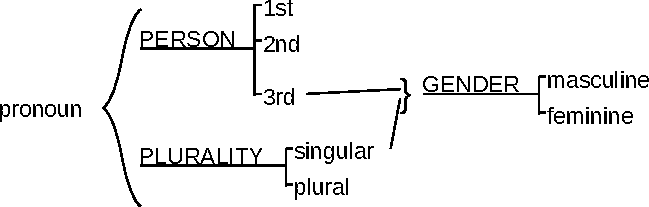
\includegraphics[width=.56\textwidth]{Figures/Example/traditional-pronoun.pdf}      
    \caption{The systematisation of three pronominal features in traditional grammar}
    \label{fig:traditional-pronoun}
\end{figure}

In SFG the pronouns are systematised in the system network of Person from \textit{Introduction to Functional Grammar} \citep[366]{Halliday2013} that has a different structure as depicted in Figure \ref{fig:person-system-network}. This systematisation reflects a semiotic perspective where language is placed into an interactive context. The (red) rectangles from the figure represent selections that are applicable to the Subject constituent ``He'' in example above. These selections are the result of traversing a system network deciding at each step which branch to follow and advance to the next system in case one is available. 

From the perspective of an agent generating the utterance in Example \ref{ex:1}, to produce the pronoun ``he'' in the subject position it has to make a few choices in the system network. This process is called system network \textit{traversal}. A simplified traversal for selecting the needed pronominal referent can be described as follows. For now, to make it simpler, the explanation on how the decissions are made is ommited focusing mainly on the traversal process itself. So, first the deciding agent chooses in the PERSON system whether the referent participates in the interaction or not (see Figure \ref{fig:person-system-network}). In our example the referent does not participate so the \textit{non-interactant} feature is selected and we proceeds towards the next system further distinguishing the type of \textit{non-interactant}. It can be plural or, as in our case, singular leading to \textit{one-referent} feature. Next, the referent needs to be differentiated on the consciousness axis which, in our example, is a \textit{conscious} thing. And finally conscious referents need to be distinguished by gender, which in this example is masculine and therefore \textit{male} sex type is chosen. This path of choices uniquely identifies the pronoun ``He'' in a system network which also defines, just like the one in Figure \ref{fig:traditional-pronoun}, the boundaries of all choice possibilities.
 
\begin{figure}[!ht]
    \centering      
    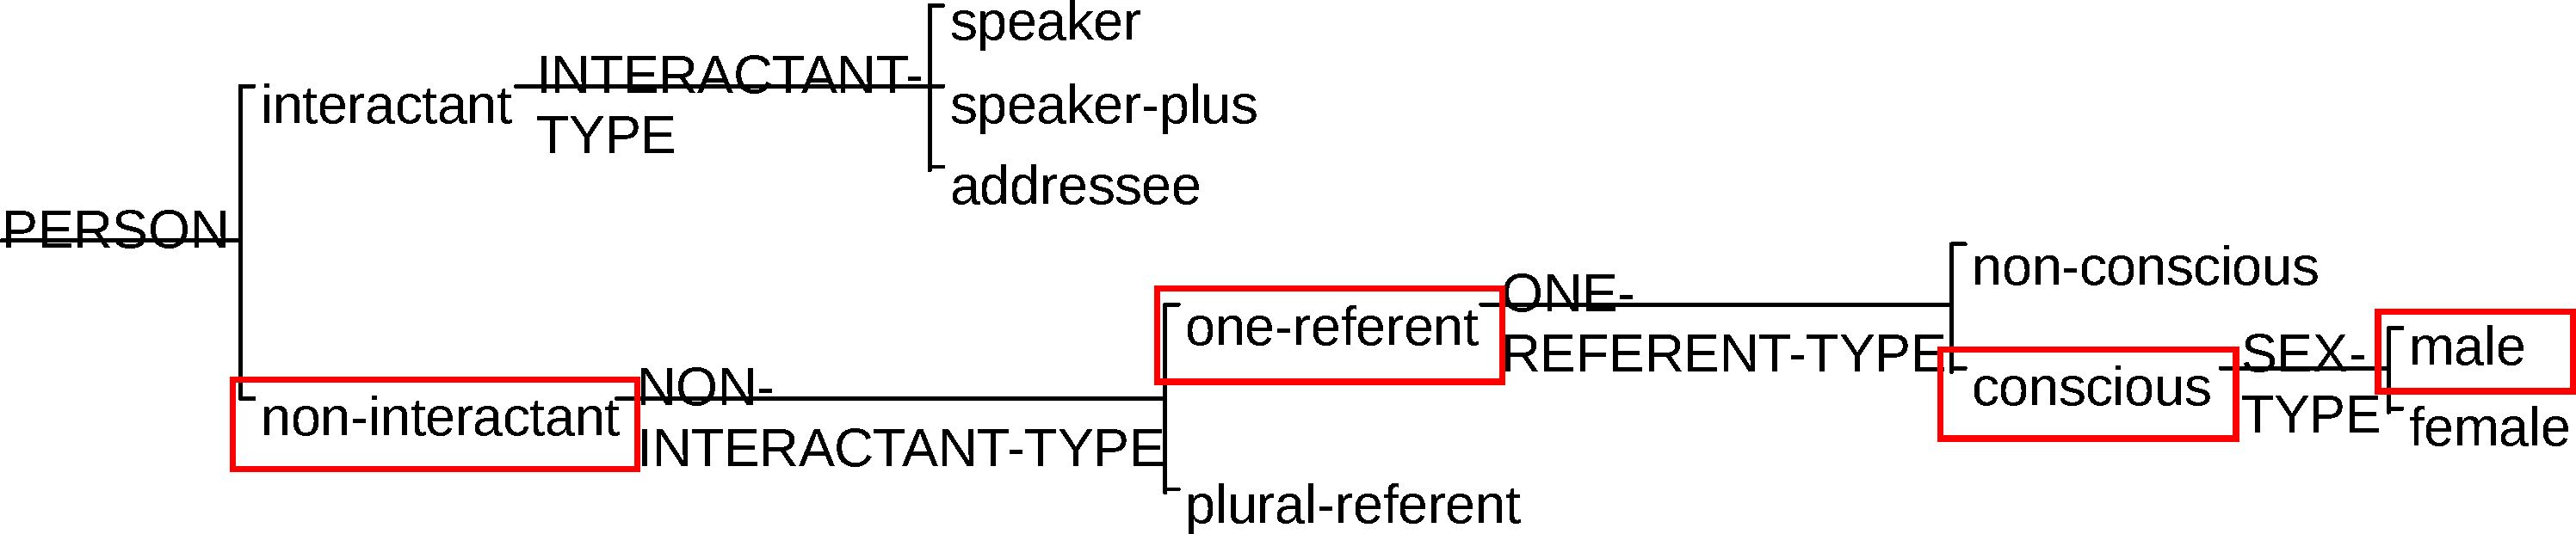
\includegraphics[width=.90\textwidth]{Figures/Example/person-selections.pdf}      
    \caption{The selections in Person system network from \citet[366]{Halliday2013} for pronoun ``He''}
    \label{fig:person-system-network}
\end{figure}

%%todo: explain how the system network is traversed and choices made, this is needed in the next section

Lets take now the clause constituent that is the root of the constituency tree (see Figure \ref{fig:constit-classes-example}) and see how SFL features can be applied to it. If in traditional grammar the clause is usually ascribed relatively few features, e.g. as having \textit{passive voice}, \textit{positive polarity} and \textit{simple past tense}; in terms of SFL grammar the corresponding features are many more i.e. \textit{major, positive, active, effective, receptive, agentive, free, finite, temporal, past, non-progressive, non-perfect, declarative, indicative, mood-non-assessed, comment-non-assessed}. Figure \ref{fig:mood-selections} depicts the selections applicable to clause constituent in Example \ref{ex:1} from Mood system network that is an adaptation of the Mood network proposed in \citet[162]{Halliday2013}. These selections represent choices made by a natural language generation system when producing the utterance by a process similar to the one explained for the pronominal referent above. The traversal description is ommited for brevity. Organisation of the linguistic features is system networks is one of the main things that distinguishes SFL from other linguistic traditions. I will formally introduce system networks, how they are structured and how they function in Chapter \ref{ch:sfg} and \ref{ch:data-structures} that follow below. 

\begin{figure}[!ht]
    \centering      
    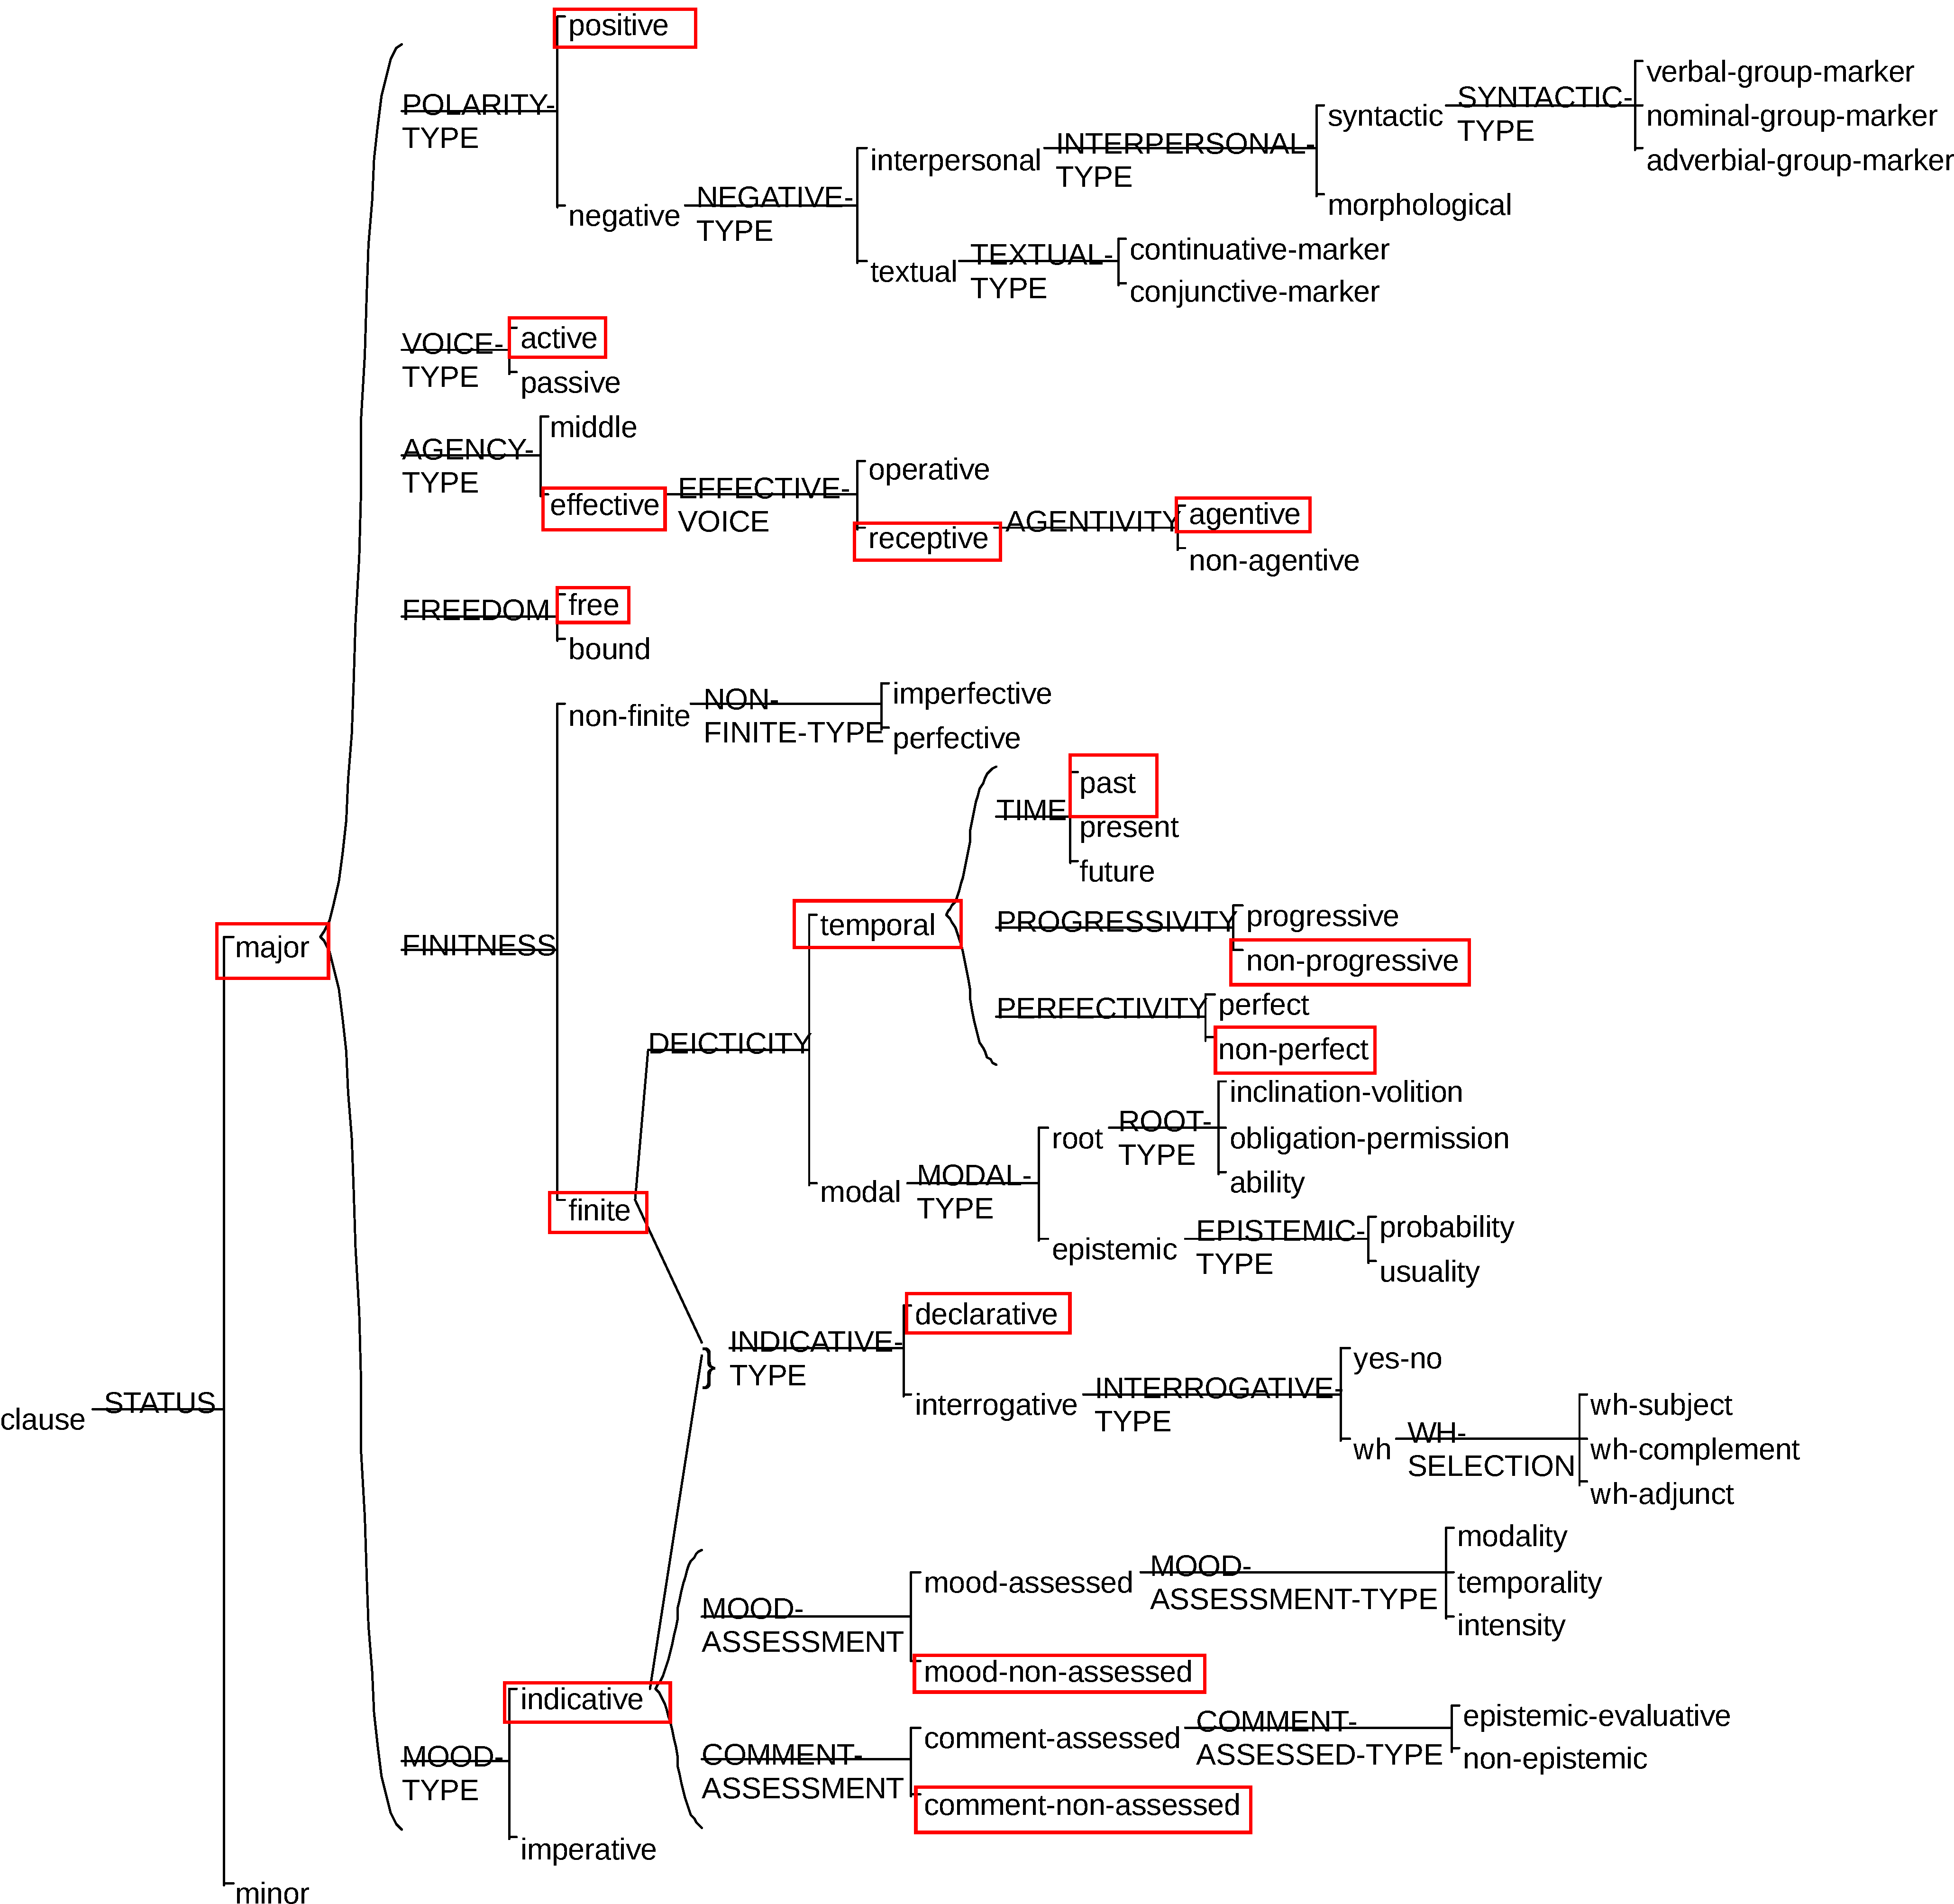
\includegraphics[width=0.91\textwidth]{Figures/Example/mood-selections.pdf}      
    \caption{The feature selections in the Mood system network for clause constituent in Example \ref{ex:1}}
    \label{fig:mood-selections}
\end{figure}

So far we have seen constituents assigned syntactic functions such as Subject, Complement, Adjunct etc. In SFL, they are elements of the \textit{interpersonal metafunction} which will be explained in Chapter \ref{ch:sfg}. SFL provides more linguistic features and functions depending on the kind of meaning it aims at describing. 
%For example what in other grammars is known as \textit{semantic labels}, \textit{thematic} or \textit{$\theta$ roles} SFL systematises as Transitivity system network (which will be introduced in Chapter \ref{sfg} below). 
For example another view on the same clause can be provided from a perspective that in SFL is called \textit{experiential} and corresponds to what in traditional linguistics is known as \textit{semantics}. It is systematised, in SFL, as Transitivity which aims at providing domain independent \textit{semantic frames} called \textit{process configurations}. They describe semantic actions and relationships, along with \textit{semantic roles} ascribed to their \textit{participants}. These semantic frames generally are ``governed'' by verbs and more specifically each verb meaning has a dedicated semantic frame.

The clause in Example \ref{ex:1} corresponds to a Possessive semantic frame where ``He'' is the Agent and Carrier while ``the cake'' is the Affected and Possessed thing. Example \ref{ex:3} provides these annotations. These configurations and participant roles correspond to the Transitivity system network proposed by \citet{Neale2002} which I will introduce in Chapter \ref{ch:the-grammar}.

\begin{exe}
    \ex\label{ex:3} [_{Agent-Carrier} He] gave [_{Affected-Possessed} the cake] away. 
\end{exe}

%%todo, move after teh next paragraph


%The analysis provided so far highlights that SFG grammar has a variety of functions serving to express different meanings. 
%The traditional grammar distinguishes them as syntactic and semantic functions but, as we will see in Chapter \ref{ch:sfg} below, SFL does not make such a distinction. Another aim of the current section was to provide a glance of the feature rich grammar and I hope the example with Mood feature selection in Figure \ref{fig:mood-selections} fulfils this goal.

\begin{figure}[!ht]
    \centering
    \begin{tikzpicture}[scale=0.8, transform shape, tree-style,
    level 1/.style={sibling distance=11em, level distance=3em,},
    level 2/.style={sibling distance=12em, level distance=3em,}, 
    edge from parent/.style={draw,rounded corners=3mm},
    anchor=north,
    edge from parent path={(\tikzparentnode.south) -- ++(0,-1em) -| (\tikzchildnode.north)},
    ]
    \node (cla) [pattern-node, split-node-31, text width = 0.9\textwidth,] 
        {He gave the cake away. 
            \nodepart{two} clause 
            \nodepart{three}  major, positive, active, effective, receptive, agentive, free, finite, temporal, past, non-progressive, non-perfect, declarative, indicative, mood-non-assessed, comment-non-assessed, posessive }
    child { node (sub)[pattern-node, split-node-3,] 
        {He 
            \nodepart{two} pronoun 
            \nodepart{three} Subject, Participant,\\ 
            Agent \& Carrier
            \nodepart{four} 3^{rd} person, singular,\\ 
            male, non-interactant,\\ 
            one-referent, conscious}}		
    child { node (mv)[pattern-node, split-node-3,] 
        {gave 
            \nodepart{two} verb 
            \nodepart{three} Main Verb, Finite, \\Process 
            \nodepart{four} %posessive
        }}
    child { node (com)[pattern-node, split-node-3,] 
        {the cake 
            \nodepart{two} nominal group 
            \nodepart{three} Complement, Participant, 
            \\ Affected \& Possessed
            \nodepart{four}
        }
        child { node (det)[pattern-node, split-node-3,] 
            {the 
                \nodepart{two} determiner 
                \nodepart{three} Deictic, Modifier
                \nodepart{four} %specific, demonstrative,\\                determinative, non-selective
            }}
        child { node (nou)[pattern-node, split-node-3,] 
            {cake 
                \nodepart{two} noun 
                \nodepart{three} Head, Thing
                \nodepart{four} %inanimate, singular,\\                 countable
            }}}
    child {node[pattern-node, split-node-3,](adjunct) 
        {away 
            \nodepart{two} adverb 
            \nodepart{three} Adjunct,
            \\Circumstance,
            \\Location
            \nodepart{four}
        }
    };
    \end{tikzpicture}
    \caption{Representation of Example \ref{ex:1} as feature rich constituency tree}
    \label{fig:mcg-graph-example}
\end{figure}

%\begin{figure}[!ht]
%    \centering
%    \begin{tikzpicture}[scale=0.8, transform shape, tree-style, 
%    level 1/.style={sibling distance=11em, level distance=14em},
%    level 2/.style={sibling distance=10em, level distance=12em}, 
%    anchor=north
%    growth parent anchor = north,]
%    
%    \node (cla) [pattern-node, split-node, text width = 42em,]  
%    {clause 
%        \nodepart{two} Configuration
%        \nodepart{three} major, positive, active, effective, receptive, agentive, free, finite, temporal, past, non-progressive, non-perfect, declarative, indicative, mood-non-assessed, comment-non-assessed, posessive};
%    
%    \node (sub) [pattern-node, split-node, below=3em of cla, xshift=-16em,] 
%    {pronoun
%        \nodepart{two} Subject, Participant,\\ 
%        Agent \& Carrier 
%        \nodepart{three} 3^{rd} person, singular,\\ 
%        male, non-interactant,\\ 
%        one-referent, conscious};
%    
%    \node (mv)[pattern-node, split-node, below=3em of cla, xshift=-5em] 
%    {verb
%        \nodepart{two} Main Verb, Finite, \\Process 
%        \nodepart{three} possessive };
%    
%    \node (com)[pattern-node,split-node, below=3em of cla, xshift=6em] 
%    {nominal group
%        \nodepart{two} Complement, Participant, 
%        \\ Affected \& Possessed
%        \nodepart{three} };
%    
%    \node (det)[pattern-node,split-node, below=3em of com, xshift=-6em]
%    {determiner
%        \nodepart{two} Deictic, Modifier
%        \nodepart{three} specific, demonstrative,\\ 
%        determinative, non-selective};
%    
%    \node (nou)[pattern-node,split-node, below=3em of com, xshift=6em]
%    {noun
%        \nodepart{two} Thing, Head
%        \nodepart{three} inanimate, singular,\\ 
%        countable };
%    
%    \node[pattern-node,split-node, below=3em of cla, xshift=17em](adjunct)
%    {adverb
%        \nodepart{two} Adjunct,
%        \\Circumstance,
%        \\Location
%        \nodepart{three} };
%    
%    \draw[sequence,-,edge-style] (cla.south) -- ++(0,-1em) -| (sub.north);
%    \draw[sequence,-,edge-style] (cla.south) -- ++(0,-1em) -| (mv.north);
%    \draw[sequence,-,edge-style] (cla.south) -- ++(0,-1em) -| (com.north);
%    \draw[sequence,-,edge-style] (cla.south) -- ++(0,-1em) -| (adjunct.north);
%    \draw[sequence,-,edge-style] (com.south) -- ++(0,-1em) -| (det.north);
%    \draw[sequence,-,edge-style] (com.south) -- ++(0,-1em) -| (nou.north);	
%    \end{tikzpicture}
%    \caption{Representation of Example \ref{ex:1} as feature rich constituency tree}
%    \label{fig:mcg-graph-example}
%\end{figure}

There are more functions and features that can be assigned to the constituents in the Example \ref{ex:1} but this is sufficient for the current purposes of introduction. Figure \ref{fig:mcg-graph-example} summarises everything discussed above into a partially filled constituency tree. The constituents that were not discussed are assigned only a few functions. %In practice, every node is richly decorated with syntactic and semantic features that are functionally anchored in the system networks.
The last (green) section of every node in the constituent tree is filled with a limited set of grammatical features selected from system networks. In practice the feature set is much richer than those shown in the nodes in Figure \ref{fig:mcg-graph-example}; the restriction aims simply to avoid an over-crowded example and simplify the exposition. Important to underline here is the systemic functional anchoring of the features into system networks that is an SFL practice.

%Generating automatically feature rich constituency structure such as the one in Figure \ref{fig:mcg-graph-example} is the general aim in the current work.

Next I describe what opportunities and limitations exist in automatically generating rich SFL analyses as until now it has not been possible to use these detailed analysis in computational contexts. This makes them unavailable for corpus work, for training data in machine learning and other end-user application scenarios provided as motivation in the Sections \ref{sec:motivation} above.

\section{Challenges of parsing with SFGs}
\label{sec:problem}
%Computing with SFG - a practical problem

%The problem of parsing with SFG has been well laid out in \citet{Bateman2008} as being one of computational complexity due to exponential explosion of possible combinations of features. 

In this sections I describe the main challenges for using Systemic Functional Grammars (SFG) in computational contexts in general and parsing in particular. The first and the main challenge in parsing with SFGs is that of computational complexity. This problem stems partially from the manner grammars are structured and partially from the fact that paradigmatic description have received most of the attention in SFL at the expense of the syntagmatic one. The second challenge is parsing with features that depart from directly observable grammatical variations towards increasingly abstract semantic features. 
%Addressing this problem required answers about a couple of other issues: the availability of a lexical-semantic database and a resolution mechanism for \textit{covert constituents}. As we will see motivated below, the latter are useful constructs in providing a solution even though some linguistic theories reject the mere existence of such things. 
Next follows a detailed description of the main problems starting with the imbalance between paradigmatic and syntagmatic accounts in SFL. Then the computational aspects are bough into the picture into as a comparison between the natural language generation and parsing tasks. Finally the problem of parsing abstract features is described drawing parallels to \textit{semantic role labelling} (SRL) task well-defined in the mainstream computational linguistics \citep{Carreras2005}. 
%Where appropriate, I will also suggesting how potential solutions may look like which will be further presented in Section \ref{sec:solution}.

\subsection{Syntagmatic descriptions in SFL}
%% the problem of syntagmatic account

Since it was established, SFL has been primarily concerned with the paradigmatic axis of language. Accounts of the syntagmatic axis of language, such as the syntactic structure, have been put in the background. Within SFL, as we will see in Chapter \ref{ch:sfg}, structure is a syntagmatic ordering in language capturing regularities and patterns which can be paraphrased as \textit{what goes together with what}. It has been placed on the theoretical map and defined in terms of \textit{rank}, \textit{unit}, \textit{class} and \textit{function}, but afterwards it received minimal attention.

Most of the descriptive work, in SFL, is carried paradigmatically via \textit{system networks} (Definition \ref{def:system}) describing \textit{what could go instead of what} \citep[22]{Halliday2013}. Having the focus set on the paradigmatic organisation in language is in fact the feature that sets SFL apart from other approaches to study language.
This has led to progress in accounting how language works at all strata but little was said about language constituency. And this can be considered ``unsolved'' within SFL accounts leaving a ``gap in what must be one the central areas of any characterisation of language'' \citep[25]{Bateman2008}. 

%Accounts of the syntagmatic axis of language, such as the syntactic structure, have been put in the background. Within SFL, structure has been placed on the theoretical map and is defined in terms of \textit{rank}, \textit{unit}, \textit{class} and \textit{function}, as we will see in detail in Chapter \ref{ch:sfg}, but afterwards it received minimal attention. 
%Most of the focus was set on 
%the paradigmatic organisation in language is in fact the feature that sets SFL apart from other approaches to study language. 
%%As we will see below, some accounts of constituency are provided within SFL grammars, enough even to make them applicable in computational domains such as automatic \textit{natural language generation}. But such descriptions are by far not satisfiable with respect to what would a proper syntagmatic account of language would be. 

If we attend SFL literature, however, the syntagmatic dimension is implicit and present everywhere in the SFL literature, which makes the above claims sound little surprising. For instance all example analyses in the \textit{Introduction to Functional Grammar} \citep{Halliday2013} are predominantly syntagmatic. 
Moreover, Robin Fawcett for decades promotes the motto \textit{no system network without realisation statements} \citep[9]{Fawcett88-good} which means that every paradigmatic description must be accompanied by precise rules how it is syntagmatically realised in text. Yet, despite these inducements, the situation could not have been more different. \citet{Bateman2008} presents in detail why there is a severe imbalance between syntagmatic and paradigmatic axes in SFL, how it came to be this way and how it is especially damaging to the task of automatic text analysis, yet quite beneficial for the text generation task. 

\subsection{Computational complexity appears in parsing}

\citet{ODonnell2005} offer a detailed description to the long history of SFL being applied in computational contexts yielding with productive outcomes on language theorising, description and processing \citep[139]{BatemanMatthiessen88}. The transfer between SFL and computation typically involved a delay between the theoretical formulation and the computational instantiation of that formulation \citep[19]{MatthiessenBateman91}. The theoretically formulated ideas contain hidden pitfalls that are revealed only upon explicit formulations required in computation \mbox{\citep[27]{Bateman2008}}. 

% def generation
The active exchange between SFL theory and computation has been almost entirely oriented towards automatic \textit{natural language generation}. Such systems take abstract semantic specifications as input and use grammars to produce grammatically correct and well-connected texts. %In the generation process the abstract semantic specifications are increasingly materialised through choice making by traversing the grammatical system network towards finally generated text (see example in Section \ref{sec:example}).

%def parsing
\textit{Automatic analysis} or \textit{parsing} can be seen as a reverse problem of finding appropriate analysis within a search space of possible solutions. That is to identify, as accurate as possible, the meaning systematised in the grammar, of a given natural language sentence. As seen in Section \ref{sec:example} above, an account of the sentence meaning would have to provide two things. First a description in terms of a formal structure of the sentence revealing the constituents plus their syntactic relations to each other. And second, a description in terms of a (complete) set of features, detailed to the extent that grammar permits, applicable to each constituent of structure. %The process starts from a given sentence and aims to derive/search the feature choices in the system network afferent to each of the constituents.

% Nigel grammar intro
One of the grammars successfully used in generation tasks is the Nigel grammar developed within Penman generation project \citep{Mann83}. The efficiency in generation tasks is, in part, due to decomposition of language along the paradigmatic axis using functionally motivated sets of choices between functionally motivated alternatives \citep{McDonald80}. The Nigel grammar contains 767 grammatical systems defined over 1381 grammatical features which Bateman evaluates as ``a very large computational grammar by current standards, although nowadays by no means the broadest when considered in terms of raw grammatical coverage'' \citep[29]{Bateman2008}.

% search and paradigmatic organisation perfect for generation
The computational processes driving natural language generation relied heavily on the notion of \textit{search}. A well defined search problem is defined in terms of a precise description of the search space which then helps a navigation process effectively to find solutions. The paradigmatic organization of the \textit{lexicogrammar} as system networks assumed within SFL turns out to organise the search space for possible grammatical units appropriate for expressing communicative goals in generation in almost ideal manner \citep[28]{Bateman2008}.

% unsuitability of paradigmatical organisation for parsing
If, in the generation process, the abstract semantic specifications are increasingly materialised through choice making by traversing the system network towards finally generated text (see example in Section \ref{sec:example}), then, in the parsing process, the reverse is the case. The process starts from a given sentence aiming to derive/search the feature choices in the system network afferent to each of the constituents. But if the paradigmatically organised lexicogrammatical resource is effective for generation it turns out, as we will see next, to be by far unsuitable for the analysis task because the size of the search space is too big to be computed in a reasonable time.
% the grammar size 
Halliday himself mentions this problem when he asks \textit{how big is a grammar?}.

\begin{quote}
    Given any system network it should in principle be possible to count the number of alternatives shown to be available. In practice, it is quite difficult to calculate the number of different selection expressions that are generated by a network of any considerable complexity \citep[10]{Halliday96-grammatics}.
\end{quote}

The issue is that of handling a combinatorial space which emerges from the way connections and (cross-)classifications are organised in a system network. In addition to that, the orientation of systemic grammars towards choice means that a typical grammar includes many disjunctions, which leads to the problem of search complexity. Also the abstract nature of systemic features leads to a structural richness that adds logical complexity to the task \citep{ODonnell1993}. So estimating the size of the grammar would in fact mean estimating the potential number of feature combinations.

For example, if we consider a hypothetical network of 40 systems then the ``size of the grammar it generates lies somewhere between 41 and 2^{40} (which is somewhere around 10^{12})'' \citep[28]{Bateman2008}. Moreover, it is not easy to calculate where would the upper limit of a grammar fall even when the configuration of relations of a particular system network is known. %One of the grammars successfully used in generation tasks is the Nigel grammar, described above, which is a large grammar by modern standards. 
%developed within Penman generation project \citep{Mann83}. It contains 767 grammatical systems defined over 1381 grammatical features which Bateman evaluates as ``a very large computational grammar by current standards, although nowadays by no means the broadest when considered in terms of raw grammatical coverage'' \citep[29]{Bateman2008}.
To parse with Nigel grammar, mentioned above, would means exploring a search space of approximately $3 \times 10^{18} $ feature combinations \citep[35]{Bateman2008}. A more detailed break down the complexity by rank or primary class as provided in Table \ref{tab:size} below.

\begin{table}[!ht]
    \centering
    \begin{tabular}{|l|r|}
        \hline
        \textit{rank or primary class} & \textit{size}                             \\ \hline
        adverbial-group                & 18                                        \\ \hline
        words                          & 253                                       \\ \hline
        quantity-group                 & 356                                       \\ \hline
        prepositional-phrase           & 744                                       \\ \hline
        adjectival-group               & 1045                                      \\ \hline
        nominal-group                  & \textgreater $ 2\times 10^{9} $  \\ \hline
        clause                         & \textgreater $ 3\times 10^{18} $ \\ \hline
    \end{tabular}
    \caption{Size of major components of the Nigel grammar expressed in terms of the number of selection expressions generated \citep[35]{Bateman2008}}
    \label{tab:size}
\end{table}

For the generation task the size is not an issue because the number of choice points is actually rather small. The paradigmatic organisation is, in fact, a concise and efficient way to express the linguistic choices where the possible feature selections are relevant only when they are enabled by prior paradigmatic choices and it is only those alternatives that need to be considered \citep[12--13]{Halliday96-grammatics}. This property of gradual exposure of choices characterises the traversal of the system networks which starts from the root and gradually advances towards more delicate features down to a leaf.

In the analysis task, the paradigmatic context of choice, that helps navigation during the generation process is no longer available. It is not known
any longer which features of a systemic network are relevant and which are not. This leads to a radical asymmetry between the two tasks. That
is: in generation, the simple traversal of the network finds only the compatible choices
because that is what the network leads to; whereas in analysis it is not evident in
advance which path to follow therefore the task is to explore the entire search
space in order to discover which features apply to the text. This means that any path is potentially relevant and shall be passed and needs to be checked leading to evaluation of the system network as a whole. There is then no way to restrict the search space as in the case of generation \citep[29]{Bateman2008}. 


\subsection{Parsing with semantic features}

%difficulty SLR
Another difficulty in parsing with SFGs lies in the fact that, as the analysis moves away from directly observable grammatical variations towards more abstract semantic variations, the difficulty of generating an accurate account increases drastically. The Transitivity system network for example consists of such semantic features and it is comparable to the task of (shallow) \textit{semantic parsing} or \textit{Semantic Role Labelling} (SRL) \citep{Carreras2005}.

The main challenge of SRL, well explained in \citep[245--250]{gildea2002automatic}, remain the same since \citet{Winograd1972}: \textit{moving away from the domain specific, hand-crafted semantic specifications towards domain independent and robust set of semantic specifications}. This goal was undertaken in several projects to build large broad-scope lexico-semantic databases such as WordNet \citep{Fellbaum98-wn}, FrameNet \citep{Baker1998, Johnson2000, fillmore2003background} and VerbNet \citep{schuler2005verbnet, Kipper2008}. A similar database exists for Transitivity system network as described in \citet{Fawcett2009} called \textit{Process Type Database} (PTDB) \citep{Neale2002}. 

Such databases provide with domain independent \textit{semantic frames} \citep{Fillmore1985}, know in SFL as \textit{configurations} or \textit{figures} e.g. Action, Cognition, Perception, Possession etc. They describe semantic actions and relationships between \textit{participants} each playing a distinct  \textit{semantic role} within the frame e.g. Agent, Carrier, Possessed, Phenomena etc. For instance the perception frame contains \textit{Perceiver} and \textit{Phenomenon} roles annotated in Example \ref{ex:glance1}.
%The semantic frames generally are governed by verbs and more specifically each verb meaning has a dedicated semantic frame. 

\begin{exe}
    \ex\label{ex:glance1} [_{Agent-Perceiver} Jaqueline] glanced [_{Phenomenon} at her new watch].
\end{exe}

%The tendency is to identify frames that are generic enough to cover classes of verb meanings (for example Action, Cognition, Perception, Possession frames) and the same applies to participant roles where the tendency is to reuse roles across semantic frames (for example agent role from Action frame is reused in Perception or Possession frames, or Phenomenon is reused in Cognition and Perception frames).

The challenge in this work is to implement a semantic parsing process for Transitivity systemic network employing PTDB as the lexical-semantic resource. 

\subsection{Covert elements}

Besides the challenge of identifying configurations and their participants in text, the problem with semantic features goes one step further. Sometimes the participant roles correspond to constituents that are displaced or not realised in the text called \textit{covert}\citep[115,135,194]{Fawcett2008} or \textit{null elements}\citep{Chomsky81, Chomsky1982, Chomsky1986}. This increases the challenge of identifying frames and assigning roles correctly and next is explained why. 
%Next I show how (non-)realisation in text of the semantic roles impacts possibility to interpret that text. Then I will show how frames may still be valid even when an element is realised or displaced which will bring us to the core of the problem. This is followed by a brief description of the approach taken in the current work to solve it.  

For a frame to be considered correctly realised in text, at least its mandatory roles must be filled by constituent units. This requirement constitutes a minimal semantic completeness constraint. This can be demonstrated by erasing parts of the text in Example \ref{ex:glance1}. If we take the Agent-Perceiver away as in Example \ref{ex:glance11} the texts is perceived as incomplete because it is not possible to interpret its meaning. It leaves us with the questions \textit{Who} glanced at her new watch? Similarly, if we delete the Phenomenon like in Example \ref{ex:glance12}, we are unable to resolve the meaning of the text without first answering the question \textit{what} or \textit{who} did Jaqueline glance at? This shows that  configurations need to satisfy the minimal semantic completeness condition when realised in text. Conversely, one of the fundamental assumptions in this work is that the input text is well-formed and the completeness condition is satisfied.

\begin{exe}
    \ex\label{ex:glance11} glanced at her new watch
    \ex\label{ex:glance12} Jaqueline glanced
\end{exe}

%example of covert constituents
Consider now Example \ref{ex:glance2} consisting of a sentence that has three non-auxiliary verbs: seem, worry and arrive. According to the Cardiff grammar (introduced in Chapter \ref{ch:sfg}) it corresponds to three clauses \textit{embedded} into each other. Table \ref{tab:glance-analsys} provides the constituency analysis in Cardiff of Example \ref{ex:glance2}.

\begin{exe}
    \ex\label{ex:glance2} She seemed to worry about missing the river boat.
%    \ex\label{ex:glance3} She seemed [to worry [about missing the river boat]].
\end{exe}

\begin{table}[!ht]
    \centering
    \resizebox{\columnwidth}{!}{%
    \begin{tabular}{cccc|c|c|c|c|c|}
        \hline
        \multicolumn{1}{|c|}{\textit{She}} & \multicolumn{1}{c|}{\textit{seemed}} & \multicolumn{1}{c|}{\textit{to}}        & \textit{worry} & \textit{about} & \textit{missing} & \textit{the} & \textit{river} & \textit{boat.} \\ \hline
        \multicolumn{9}{|c|}{clause}                                                                                                                                                                                              \\ \hline
        \multicolumn{1}{|c|}{Subject}      & \multicolumn{1}{c|}{Main Verb}       & \multicolumn{7}{c|}{Complement}                                                                                                               \\ \hline
        & \multicolumn{1}{c|}{}                & \multicolumn{7}{c|}{clause}                                                                                                                   \\ \cline{3-9} 
        & \multicolumn{1}{c|}{}                & \multicolumn{1}{c|}{Infinitive Element} & Main Verb      & \multicolumn{5}{c|}{Complement}                                                    \\ \cline{3-9} 
        &                                      &                                         &                & \multicolumn{5}{c|}{clause}                                                        \\ \cline{5-9} 
        &                                      &                                         &                & Binder         & Main Verb        & \multicolumn{3}{c|}{Complement}                \\ \cline{5-9} 
    \end{tabular}%
    }
    \caption{SF constituency analysis in Cardiff grammar style of Example \ref{ex:glance2}}
    \label{tab:glance-analsys}
\end{table}

Table \ref{tab:semantic-role-distro} provides the participant role configurations (i.e. the semantic frames) these verb meanings bring about. Usually the first role corresponds to the Subject function and the second role is filled by a Complement unit.
%For the sake of this example the first role corresponds to the Subject constituent and the second to the Complement constituent. This way 

The verb meaning \textit{seem_{1}} corresponds to an Attributive configuration that distributes Carrier and Attribute roles to the Subject ``She'' and the Complement ``to worry about missing the river boat''. In the case of \textit{worry about_1} and \textit{miss_1} the first roles provided by Cardiff grammar are \textit{compound} i.e. composed of two simple ones. %, while the second ones are simple. 
In the example above, \textit{worry about_1} distributes the Phenomenon to the Complement ``about missing the river boat'' and the Agent-Cognizant role to an empty Subject that is said to be \textit{non-realised}, \textit{covert} or \textit{null element}. A similar situation is for \textit{miss_1} that assigns an Affected-Carrier role to the empty Subject and the Possessed role to the Complement ``the river boat''. 

\begin{table}[!ht]
    \centering
    \begin{tabulary}{0.95\textwidth}{|c|C|C|}
        \hline
        \textbf{Verb meaning} & \textbf{Semantic configuration} & \textbf{Participant role distribution}  \\ \hline
        \textit{seem_{1}}           & Attributive                     & Carrier + Attribute                     \\ \hline
        \textit{worry about_{1}}   & Two Role Cognition              & Agent-Cognizant + Phenomenon         \\ \hline
        \textit{miss_{1}}           & Possessive                      & Affected-Carrier + Possessed (thing) \\ \hline
    \end{tabulary}
    \caption{Semantic role configurations according to \citet{Neale2002,Fawcett2009}}
    \label{tab:semantic-role-distro}
\end{table}

Those unrealised Subjects in the embedded clauses are recoverable from the immediate syntactic context (no need for discourse) and correspond, in this case, to the Subject in the higher clause. This is annotated in Examples \ref{ex:glance3} and \ref{ex:glance4} therefore we can just mark the places of the null Subjects in the embedded clause in order to be able to assign the semantic labels this way ensuring that the minimal completeness constraint is fulfilled; otherwise the frame cannot be assigned to the constituents and another one shall be searched for instead. Notice also an index \textit{i} to highlight that the null elements correspond to the higher clause Subject ``She''. 

\begin{exe}
    \ex\label{ex:glance3} \textit{She} worried about missing the river boat.
    \ex\label{ex:glance4} \textit{She} missed the river boat.
    \ex\label{ex:glance5} She_i seemed [\textit{null-Subject}_i to worry [about \textit{null-Subject}_i missing the river boat]].
\end{exe}

Now that the places of the covert constituents are explicitly marked in Example \ref{ex:glance5} and the recoverable constituents coindexed we can distribute the semantic role configurations from Table \ref{tab:semantic-role-distro} as provided in Table \ref{tab:glance-analsys-semantic} below. 

\begin{table}[!ht]
    \centering
    \resizebox{\textwidth}{!}{%
        \begin{tabular}{cccccc|c|c|c|c|c|}
            \hline
            \multicolumn{1}{|c|}{\textit{She_i}}   & \multicolumn{1}{c|}{\textit{seemed}} & \multicolumn{1}{c|}{$\emptyset_i$}   & \multicolumn{1}{c|}{\textit{to}} & \multicolumn{1}{c|}{\textit{worry}} & \textit{about} & $\emptyset_i$ & \textit{missing} & \textit{the} & \textit{river} & \textit{boat.} \\ \hline
            \multicolumn{11}{|c|}{Attributive configuration}                                                                                                                                                                                                                         \\ \hline
            \multicolumn{1}{|c|}{Agent} & \multicolumn{1}{c|}{}       & \multicolumn{9}{c|}{Attribute}                                                                                                                                                                               \\ \cline{1-1} \cline{3-11} 
            & \multicolumn{1}{c|}{}       & \multicolumn{9}{c|}{Two role cognition configuration}                                                                                                                                                        \\ \cline{3-11} 
            & \multicolumn{1}{c|}{}       & \multicolumn{1}{c|}{Agent \& Cognizant} &                         & \multicolumn{1}{c|}{}               & \multicolumn{6}{c|}{Phenomenon}                                                                       \\ \cline{3-3} \cline{6-11} 
            &                             &                                      &                         & \multicolumn{1}{c|}{}               & \multicolumn{6}{c|}{Possessive configuration}                                                         \\ \cline{6-11} 
            &                             &                                      &                         &                                     &                & Affected \& Carrier &                  & \multicolumn{3}{c|}{Possessed}                 \\ \cline{7-7} \cline{9-11} 
        \end{tabular}%
    }
    \caption{Transitivity analysis in Cardiff grammar style \citep{Neale2002,Fawcett2009} of Example \ref{ex:glance2}} 
    \label{tab:glance-analsys-semantic}
\end{table}

In language there are cases where constituents are empty but recoverable from the immediate vicinity by relying in most cases on syntactic means and in a few others additional lexical-semantic resources are needed.
In SFL, Fawcett describes these elements in the context of Cardiff grammar \citep[115,135,194]{Fawcett2008} but provides no means to recover them. The Government and Binding Theory (GBT) developed in \citep{Chomsky81, Chomsky1982, Chomsky1986} and based on phrase structure grammar, provides a detailed account of mechanisms to detect and resolve the empty constituents. GBT explains how some constituents can \textit{move} from one place to another, where are the places of \textit{non-overt constituents} and what constituents do they refer to i.e. what are their \textit{antecedents}. Such accounts of empty elements are useful in determining the correct distribution of participant roles to the clause constituents.
%are missing from any SFG grammar and can be integrated into SFG to aid the Transitivity analysis.
% This is especially valuable in the SRL task for automatically determining the correct distribution of participant roles to the clause constituents.
%Translating the mechanisms from GBT into SFG could contribute to decreasing the complexity of the parsing problem mentioned above.

% concluding problem
\subsection{Problem summary}

This section has shown the main challenges related to parsing with SFG which can be summarised as follows. 
First, the parsing task cannot be treated as a reversible generation task because the methods that have been shown to work for generation are not usable for parsing as such due to a high computational complexity. Second, the parsing task, regardless of the grammar, should first and foremost account for the sentence structure on the syntagmatic axis and only afterwards for the (semantic) features selected on the paradigmatic axis. Such syntagmatic account in SFL is insufficient for the parsing task. Third, syntagmatic account alone does not provide enough clues for assignment of semantic features and requires a lexical-semantic account within the grammar or as separate resource. Moreover, semantic parsing can be aided by identification of places where covert constituents are said to exist. %Identifying such the null elements is not the only method of assigning semantic features and some approaches do without them but having access to such information is considered valuable in the present thesis.

Next I will describe how these problems have been addressed in the current work, what are the goals of the thesis and what has been left out for the future work.

%% some sugestions 
%Regarding the problem of computational complexity explained above, how could the large search space of grammars such as Nigel be restricted to a reasonable size and how can be compensated the lack of proper syntagmatic description in SFGs? The first part of the question has already been addressed in \citet{ODonnell1993} in at least what would a possible solution look like. 

%
%Therefore to address parts of the above problems I attempt a different approach. %which is \textit{reuse} of positive results. 
%Some linguistic frameworks, other than SFL, have been shown to work well in computational contexts solving problems similar to the ones identified above. For the purposes of this thesis I selected Dependency Grammar (DG) and GBT. And instead of attempting to find novel solutions within the SFL framework, an alternative approach, I argue in the next section, would be to establish a cross-theoretical and inter-grammatical links and to enable integration of the ready solutions. 

\section{Goals and scope of the thesis}
\label{sec:solution}
%Thesis Goals and Proposed Solution

This thesis aims at a modular method for parsing unrestricted English text into a Systemic Functional constituency structure using fragments of Systemic Functional Grammar (SFG) and dependency parse trees.

The computational complexity, the lack of proper syntagmatic description in SFL and perhaps for other hidden reasons the results of parsing with SFGs so far are not usable in real world applications. This conclusion is drawn from the past attempts such as \citet{Kasper1988}, \citet{Kay1985}, \citet{ODonoghue1991a}, \citet{ODonnell1993} and \citet{Day2007}, to mention just a few, none of which managed to parse broad coverage English with full SFG without aid of some sort. A detailed account of the current state of the art in parsing with SFGs is provided in Chapter \ref{ch:sota}. Some parsing approaches use a syntactic backbone which is then flashed out with an SFG description. Others use a reduced set or a single layer of SFG representation; and the third group use an annotated corpus as the source of a probabilistic grammar. Each had to accept limitations either in grammar or language size and eventually used simpler syntactic trees as a starting point.% of the parsing process called parsing with a syntactic backbone.

%Regardless of approach, each limits the SFG in one way or another, balancing the depth of description with language coverage: that is either \textit{deep description but a restricted language} or \textit{shallow description but broad language coverage} is attempted. The current thesis tilts towards the latter: while keeping the language coverage as broad as possible the aim is to provide, in the parse result, as many systemic features as possible.

Some linguistic frameworks, other than SFL, have been shown to work well in computational contexts solving problems similar to the ones identified above. For the purposes of this thesis I selected Dependency Grammar (DG) and GBT. And instead of attempting to find novel solutions within the SFL framework, an alternative approach, I argue in the next section, is to establish a cross-theoretical and inter-grammatical links and to enable integration of the existing methods, resources and solutions in order to maximise reuse of positive outcomes.

The process developed in this thesis follows a pipeline architecture (see Section \ref{sec:architecture}) comprising of two major phases: the \textit{structure creation} and the \textit{structure enrichment}. The structure creation phase aims to account for the syntagmatic dimension of language. %Here a syntactic backbone is created from the Stanford dependency grammar parse graphs. 
The structure enrichment phase aims at discovering and assigning systemic features (accounting for the paradigmatic dimension of language) afferent to each of the nodes constituting the structure. 


%In this phase, two kinds of feature enrichments can be distinguished by the kinds of clues used for feature identification. The first kind of clues are syntagmatic (constituency tree, unit class, unit function, linear order, position) and can be detected using, what I call, the \textit{structural patterns} while the second kind of clues are lexical-semantic requires lexical-semantic and potentially more kinds of resources in addition to the structural patterns.

\subsection{On theoretical compatibility and reuse}
\label{sec:reuse}
%on theoretical compatibility and reuse
% reuse motivation, context to parsing 
In the past decades much significant progress has been made in natural language parsing framed in one or another linguistic theory each adopting a distinct perspective and set of assumptions about language. The theoretical layout and the available resources influence directly what is implemented into the parser and each implementation approach encounters challenges that may or may not be common to other approaches in the same or other theories. 

Parsers implementing some theoretical framework may face common or different challenges to those implementing another theoretical frameworks. The converse can be said of the solutions. When a solution is achieved using one framework it becomes potentially reusable in other ones provided a degree of adaptation. Thus the successes and achievements in any school of thought can be regarded as valuable for other ones to the degree cross theoretical links and correspondences can be established. In this thesis reusing components that have been shown to work and yield ``good enough results'' is a strong pragmatic motivation in the present work which brings us to Research question \ref{question:reuse-broad}.

\begin{question}[Reuse positive results]\label{question:reuse-broad}
    To what extent resources and techniques from other areas of computational linguistics can be reused for the SFL parsing and how?
\end{question}

In this thesis three linguistic frameworks are employed, namely the \textit{Systemic Functional Linguistics}, \textit{Dependency Grammar} and \textit{Governance \& Binding Theory}. SFL has already been motivated as target analysis framework in Section \ref{sec:framework}. The other two frameworks are employed because the accomplishments in those domains carry answers to above stated problems. %The goal is to maximise their positive properties and enable reusing the existing results.

%The compatibility
%It demonstrates how selected grammatical frameworks namely \textit{Systemic Functional Grammar}, \textit{Dependency Grammar} and \textit{Governance \& Binding Theory} relate to each other and to which degree they are compatible to undergo a conversion process and to show that simple patterns carrying grammatical information can be used to enrich syntactically and semantically the parse structures. And here is a brief motivation for selecting these frameworks.   

%
In the past decade \textit{Dependency Grammar} \citep{Tesniere2015} has become quite popular in natural language processing world favoured in many projects and systems. The grammatical lightness and the  modern algorithms implemented into dependency parsers such as Stanford Dependency Parser \citep{Marneffe2006}, MaltParser \citep{Nivre2006}, MSTParser \citep{McDonald2006} and Enju \citep{Miyao2005} are increasingly efficient and highly accurate. Among the variety of dependency parsing algorithms, a special contribution bring the \textit{machine learning} methods such as those described in \citet{mcdonald2005online, mcdonald2006online, carreras2007experiments, zhang2011transition, pei2015effective} to name just a few. 

\begin{question}[Compatibility of DG and SFG]\label{question:reuse-dg}
    To what degree the syntactic structures of the Dependency Grammar and Systemic Functional Grammar are compatible to undergo a transformation from one into the other?
\end{question}

The dependency parse structures provide information about functional dependencies between words and grants direct access to the predicate-argument relations. %and can be used off the shelf for real world applications. 
This information is sufficient to supplement the missing syntagmatic account in SFL. In addition, it provides some functional information that helps to reduce the complexity of system network traversing. 
This hypothesis, formulated as Research question \ref{question:reuse-dg}, is investigated at the theoretical level in Chapter \ref{ch:dependecy-grammar} and then empirically evaluated in Chapter \ref{ch:evaluation} based on Stanford Dependencies parser version 3.5 \citep{Marneffe2008a,Marneffe2008, Marneffe2014}.  

%One of the goals, as formulated in Research question \ref{question:reuse-dg}, is to investigate to which degree the dependency grammar is structurally and functionally compatible with SFGs to undergo a cross theoretic transformation. This hypothesis is investigated  

\begin{question}[Compatibility of GBT and SFG]\label{question:reuse-gbt}
    How can Government and Binding Theory be used for detecting places of null elements in the context of SFL constituency structure?
\end{question}

%In Section \ref{question:reuse-gbt} above was motivatyed and explained the need to place the empty elements into the structure in order to facilitate Transitivity analisys. GBT is well known to deal and explain mechanisms for acheiving this goal on 

The problem of accounting for the \textit{null elements}, mentioned above, is not addressed either in SFL or in Dependency Grammar. It is, however, addressed in detail in the Government and Binding Theory (GBT) \citep{Chomsky81,Haegeman1991} which is one of Chomsky's Transformational Grammars \citep{Chomsky1957}. One other goal in this thesis is to investigate, as formulated in Research question \ref{question:reuse-gbt}, to which degree GBT accounts of null elements can be reused as DG or SFG structures to undergo a cross-theoretic transformation enabling those accounts in DG or SFG contexts. Chapter \ref{ch:gbt} introduces GBT and investigate this hypothesis providing some of the cross-theoretic and inter-grammatical links to Dependency and SFL grammars that as we will see in Chapter \ref{ch:enrichment-stage} benefits the Transitivity analysis.

%Chapter \ref{ch:dependecy-grappamr} and \ref{ch:gbt} besides introducing the Dependency grammar and correspondingly Government and Binding Theory show how these frameworks relate to each other and to which degree they are compatible to undergo a conversion process for the purpose of reuse.

\subsection{Towards the syntagmatic account}
\label{sec:syntagmatic-account}
%solution to syntagmatic deficit
%The problem in using SFGs for parsing, as we have seen in Section \ref{sec:problem} above, manifests when the grammar is instantiated computationally with a primary focus on paradigmatic organisation (prevalent in SFL) at the cost of syntagmatics which leads to the first difficulty that needs to be addressed: discovering from a sequence of words what possible groups are combinable into grammatical groups, phrases or clauses. This is a task of bridging a sequence of words as input and the grammatical description of how they can combine to form a (syntactic) constituency tree structure (known in SFL as \textit{syntagmatic organizations} which will be addressed in Section \ref{sec:structure-sydney}). 

%This challenge will be addressed by filling the gap of the syntagmatic account within the SFL grammar directly. This involves, first, providing information about which grammatical functions operate at each rank, second, which grammatical functions can be filled by which classes of units and, third, providing relative and absolute description of the element order for each unit class. This information in the grammar can guide the process of building the constituency structure. 

The problem of structure construction can be outsourced as parsing with other grammars. This is done in the works of Kasper \citet{Kasper1988} and \citet{Honnibal2004a, Honnibal2007} who used phrase parse structures of the Chomskian style grammars. This approach is knows in SFL literature as \textit{parsing with a syntactic backbone}. In this case, the problem changes into creating a transformation mechanism to obtain the SFL constituency structure rather than build it from scratch. 

%Starting the SFG parsing process from a syntactic tree produced with other grammars reduces the computational complexity and the search space discussed in Section \ref{sec:problem} above. 

\begin{question}[Suitability of Stanford DG]\label{question:reuse-stanford}
    How compatible are the grammatical categories and practices in the Stanford Dependency grammar with the ones in Parsimonious Vole grammar?
\end{question}

This thesis addresses the problem of constituency structure building by parsing the text with Stanford Dependencies parser version 3.5 \citep{Marneffe2008a,Marneffe2008, Marneffe2014} and then transforming the parse result into SFG constituency tree. The degree to which Stanford dependecies are suitable to serve as a syntactic backbone is one of the questiosn adressed in this thesis (Research question \ref{question:reuse-stanford}). % which requires beforehand a theoretical discussion in terms of what is being transformed (expressed in Research question \ref{question:reuse-dg}).
An account of correspondence between linguistic primitives or configurations of primitives in the dependecy grammar to SFG primitives is provided in the end of Chapter \ref{ch:dependecy-grammar} along with an analisys of Stanford dependecy grammar. The detailed description of the structure generation process is provided in the Chapter \ref{ch:parsing-algorithm}.

%Furthermore, the constituency structures is generated through a process that involves: traversing the source (dependency) parse tree and, at each traversal step, executing a constructive operation on a parallel tree following a predefined rule set of operations and mapping relations. The detailed description of the structure generation process is provided in the Chapter \ref{ch:parsing-algorithm}. 

\subsection{Towards the paradigmatic account}
\label{sec:paradigmatic-account}
%todo continue here
Once the constituency structure is in place it serves as foundation and informs the following process of feature enrichment. The configurations of units carrying grammatical categories and functions into \textit{structural patterns} serve as ``hooks'' to guide the traversal of system networks in a way resembling the realization rules. %the paradigmatic context available during the generation process. 
%Such configurations resemble the SFG \textit{realization rules} which, during the generation process, instantiate the (abstract) features as text.

\begin{figure}[!ht]
    \centering      
    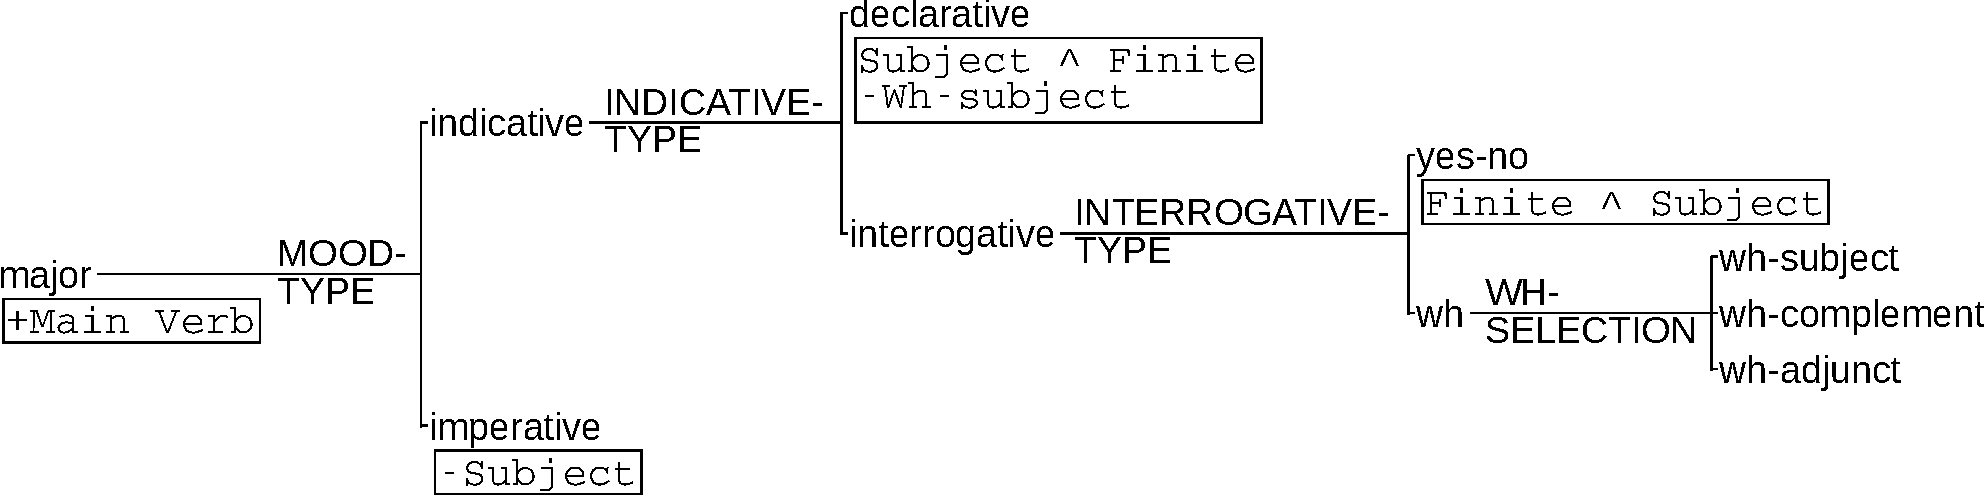
\includegraphics[width=0.91\textwidth]{Figures/Example/just-mood.pdf}      
    \caption{A fragment of mood system from \citet[366]{Halliday2013}}
    \label{fig:just-mood}
\end{figure}

The system network fragment in Figure \ref{fig:just-mood} contains the realisation rules inscribed into rectangular boxes positioned below some features. These realisation rules indicate what shall be reflected in the structure when a feature is selected (discussed already in Section \ref{sec:problem}). The converse is also true: if structure contains a certain pattern then it is a (potential) manifestation of a given feature. 

For example the structure of a \textit{major} clause needs to have a predicate or Main Verb element realised. In the parsing process, testing whether there is a unit functioning as Main Verb below in the clause node suffices to assign the \textit{major} feature to that clause. Next, if the clause has no unit functioning as Subject then it shall be assigned \textit{imperative} feature otherwise the \textit{indicative} one. Further the INDICATIVE-TYPE system is enabled. Here the test is whether a Subject node is positioned in front of the Finite node and whether the Subject contain the preposition ``who''. This sort of queries on the structure can be formulated as \textit{structure patterns} (see Section \ref{sec:pattern-graphs}) and associated to features in the system network in the same manner the realisation rules are. 

Such paterns can be identified in the instance structure and therefore the specific feature. In current parsing method, pattern recognition plays an essential role for fleshing out the constituent backbone with systemic features. The structural patterns are tested whether they \textit{match} (see Section \ref{sec:pattern-graph-matching}) anywhere in the constituency structure and if so then the matched nodes are enriched with the features proved in the pattern (described in Section \ref{sec:pattern-based-operations}). This process is detailed in Section \ref{sec:enrichment-stage}. 

The structure patterns in this work are expressed as \textit{graph patterns} (described in Section \ref{sec:pattern-graphs}). Note that I employ the concept of \textit{graph} and not that of a tree because the latter are too restrictive for the purpose of the current work. While most of the time they are hierarchically structured as a tree there are few patterns that involve sibling connections or nodes with multiple parents. In both cases the tree structure is broken. The graph construct allows a wide range of structural configurations including the trees. This comes with the cost of higher computation power thus subject for optimisations in the future work. 

%The enrichment stage of the parsing process comprises of a series of graph pattern matching operations that in case of success leads to the enrichment of the constituency structure with the features given in the graph pattern. This mechanism is described in detail in the Section \ref{sec:enrichment-stage}. 

Most of the graph patterns in this work have been manually created. Because this is laborious exercise only a few system networks have been covered in the implementation of the parser. Nonetheless they suffice for deriving some conclusions regarding the parsing approach. The future work may investigate how can graph patterns be generated automatically from the realisation rules of large grammars such as Nigel. 

\begin{question}[Coverage of syntactic patterns]\label{question:pattern-delicacy}
    What degree of systemic delicacy can be reached using syntactic patterns alone without any lexical-semantic resources?
\end{question}

The pattern may comprise solely of syntactic specifications or it can also carry lexical-semantic descriptions. 
%The two differ in the way they are generated and maintains therefore an investigation of how many features can be expressed in terms of sole syntactic configurations is important. 
The two main system networks targeted in this work are MOOD and TRANSITIVITY (described in Chapter \ref{ch:the-grammar}). One hypothesis formulated in Research question \ref{question:pattern-delicacy} is that the MOOD network is composed of syntactically identifiable features thus the graph patterns need to involve no more than unit classes and functions available in the constituency structure. 

\begin{question}[PTDB suitability]\label{question:ptdb-suitable}
    How suitable is Process Type Database as a resource for SFL Transitivity parsing? 
\end{question}


The TRANSITIVITY network requires a lexical-semantic database in order to derive graph patterns. This work employs the Process Type Database (PTDB) \citep{Neale2002} to aid generation of such patterns. The appropriateness of PTDB for these tasks is inquitred by Research question \ref{question:ptdb-suitable} and addressed in Chapters \ref{ch:the-grammar} and \ref{ch:enrichment-stage}. In the next section is presented an overview of how these processes fit together in a unitary pasing process.

\subsection{Parsimonious Vole architecture}
\label{sec:architecture}
The current thesis is accompanied by a software implementation called the Parsimonious Vole parser. It is programmed with Python language and is available as open source distribution\footnote{\url{https://bitbucket.org/lps/parsimonious-vole}}. It takes the text of an English sentence as input and outputs the rich systemic functional constituency structure. This section explains the implemented parsing process architecture.

The parser follows the pipeline architecture depicted in Figure \ref{fig:pipeline-overview}. Three types of boxes are used here: (a) the red rounded rectangles in the middle represent parsing steps, (b) the green trapezoid boxes represent input and output data and (c) the orange double framed trapezoid boxes represent external resources involved in the parsing process e.g. system network, graph patetrns, lexical-semantic databases etc. 

The parsing steps linearly flow from one to the next via green trapezoid boxes on the left-hand side of the diagram. It means that the output data of a step constitutes the input for the next one. On the right-hand side are positioned double edged orange trapezoids representing fixed resources needed by some operations. For example, the \textit{graph normalization} step takes a set of graph patterns that serve as normalisation rules indicating how to update the input.

Two green vertical arrows are provided on the far right of the diagram delimiting parsing phases: \textit{Graph Building} (spanning the first three process steps) that accomplishes construction of the constituency backbone (motivated in Section \ref{sec:syntagmatic-account} above) and the second phase \textit{Graph Enrichment} (spanning the last three process steps) flashes out the backbone with features (motivated in Section \ref{sec:paradigmatic-account}).

\begin{figure}[!ht]
    \begin{tikzpicture}[node distance=1.2em, scale=0.85, transform shape]
    % aLVL 0
    \node[](data) {}; % invisible node
    \node[right=12em of data](process) {}; % invisible node
    \node[right=12em of process](resource) {}; % invisible node 
    \node[right=9.5em of resource](flow) {}; % invisible node 
    
    % aLVL 1
    \node[data,anchor=center, below=-2em of data] (text) {Input Text};
    \node[task,anchor=center, below=-2em of process] (dep-parse) { Dependecy Parsing};
    \draw[sequence,->] (text) -- (dep-parse);
    
    % aLVL 2
    \node[data,anchor=center, below=6.5em of data] (dep-graph) {Dependecy Graph};
    \node[task,anchor=center, below=6em of process] (correction) {Error Correction \& \\ Graph Normalization};
    \draw[sequence,->] (dep-graph) -- (correction);
    \draw[sequence,->] (dep-parse.south) -- ++(0,-1.5em)  -| (dep-graph.north);
    
    % resources
    \node[persistent-data,anchor=center, below=4em of resource] (error-graph) {Common Error \\ Graph Patterns};
    \node[persistent-data,anchor=center, below=8em of resource] (norm-graph) {Normalization \\ Graph Patterns};
    
    \draw[sequence,->] (error-graph.west) -- ++(-1.5em,0)  |- (correction.east);
    \draw[sequence,->] (norm-graph.west) -- ++(-1.5em,0)  |- (correction.east);
    
    % aLVL 3
    \node[data,anchor=center, below=14em of data] (norm-dep-graph) {Normalised \\ Dependency Graph };
    \node[task,anchor=center, below=14em of process] (const-cr) {Constituency Graph \\ Creation};
    \draw[sequence,->] (norm-dep-graph) -- (const-cr);
    \draw[sequence,->] (correction.south) -- ++(0,-1.5em)  -| (norm-dep-graph.north);
    
    % resources
    \node[persistent-data,anchor=center, below=14.22em of resource] (rule-table) {Rule Table}; % 12.425
    \draw[sequence,->] (rule-table.west) --  (const-cr.east);
    
    % aLVL 4
    \node[data,anchor=center, below=24em of data] (const-gr) {Constituency Graph };
    \node[task,anchor=center, below=23.5em of process] (const-gr-enr) {Mood\\Enrichment};
    \draw[sequence,->] (const-gr) -- (const-gr-enr);
    \draw[sequence,->] (const-cr.south) -- ++(0,-1.5em)  -| (const-gr.north);
    
    %resources
    \node[persistent-data,anchor=center, below=21em of resource] (sys-net) {System Network};
    \node[persistent-data,anchor=center, below=23.5em of resource] (feat-dict) {Feature-rich \\ Dictionaries};
    \node[persistent-data,anchor=center, below=27em of resource] (sys-feat-gm) {Mood \\ Graph Patterns};
    \draw[sequence,->] (feat-dict.west) --  (const-gr-enr.east);
    \draw[sequence,->] (sys-net.west) -- ++(-.79em,0)  |- (const-gr-enr.east);
    \draw[sequence,->] (sys-feat-gm.west) -- ++(-1.9em,0)  |- (const-gr-enr.east);
    
    % aLVL 5
    \node[data,anchor=center, below=31.5em of data] (enriched-gr) {(Feature Enriched) \\ Constituency Graph };
    \node[task,anchor=center, below=31.5em of process] (null-cr) {Null Element \\ Creation};
    \draw[sequence,->] (enriched-gr) -- (null-cr);
    \draw[sequence,->] (const-gr-enr.south) -- ++(0,-1.5em)  -| (enriched-gr.north);
    
    %resources
    \node[persistent-data,anchor=center, below=31.5em of resource] (null-gr) {Null Element \\ Graph Patterns};
    \draw[sequence,->] (null-gr) -- (null-cr);
    
    %aLVL 6
    \node[data,anchor=center, below=38.5em of data] (null-enr-gr) {(Null Enriched) \\ Constituency Graph };
    \node[task,anchor=center, below=38.5em of process] (sem-enr) {Transitivity \\ Enrichment};
    \draw[sequence,->] (null-enr-gr) -- (sem-enr);
    \draw[sequence,->] (null-cr.south) -- ++(0,-1.5em)  -| (null-enr-gr.north);
    
    %resources 
    \node[persistent-data,anchor=center, below=36em of resource] (sys-net1) {System Network};
    \node[persistent-data,anchor=center, below=38.5em of resource] (ptdb) {Process Type \\ Database};
    \node[persistent-data,anchor=center, below=42em of resource] (pc-gp) {Transitivity \\ Graph Patterns};
    \draw[sequence,->] (sys-net1.west) -- ++(-1.35em,0)  |- (sem-enr.east);
    \draw[sequence,->] (pc-gp.west) -- ++(-2.4em,0)  |- (sem-enr.east);
    \draw[sequence,->] (ptdb.west) -- (sem-enr.east);
    
    %aLVL 7
    
    \node[data,anchor=center, below=45em of data] (final) {Rich Constituency Graph};
    \draw[sequence,->] (sem-enr.south) -- ++(0,-1.5em)  -| (final.north);
    
    % vertical arrows
    
%    \node[flow-arrow, below=-2em of flow] (bootstrapping) {Bootstrapping};
%    \node[flow-arrow, below=7em of flow] (pre-processing) {Pre-processing};
%    \node[flow-arrow, below=15em of flow] (creation) {Graph \\ Building};
    \node[flow-arrow, below=7em of flow, minimum width=22em] (building) {Graph Building};
    \node[flow-arrow, below=32.5em of flow, minimum width=26em] (enrichment) {(Increasingly Semantic) Graph Enrichment};
    \end{tikzpicture}
    \caption[]{The parsing process pipeline}
    \label{fig:pipeline-overview}
\end{figure}

%One important feature of this implementation is its heavy reliance on graph pattern matching and other operations using graph patterns described in Chapter \ref{ch:data-structures}. 

The parsing process starts with from an English text which is sent to Stanford Dependency parser \citep{chen2014fast} version 3.5\footnote{\url{https://nlp.stanford.edu/software/nndep.html}} to produce a Dependency parse graph of that text. The output is a sequence of dependency graphs corresponding to sentences delimited by punctuation marks.

The dependency graphs often contain errors. Some of these errors are predictable and so easy to identify and correct. Also, some linguistic phenomena are treated in a slightly different manner than that proposed in the current thesis. Therefore, dependency graphs produced by the Stanford parser are \textit{Corrected and Normalised} against a collection of known errors and a set of normalisation rules using pattern matching techniques.

Afterwards, the normalised dependency graph is ready to guide the \textit{building process} of the systemic functional constituency graph. Through a traversal of the dependency graph the constituency graph is constructed in parallel guided by a \textit{Rule Table}. This table contains the mapping of structural context fragments from the dependency grammar (i.e. node type, edge type, combinations of the two etc.) to constituency graph nodes. The structural mappings are accompanied by operation specifications to perform during each traversal step. The output of this step constitutes the syntactic backbone on which the subsequent enrichment phases are performed.

Next follows the phase where each constituent node of the syntactic backbone is \textit{enriched} with features. Some of them are syntactic in nature and others are lexical-semantic. In between these enrichment phases there is an additional construction process adding where needed \textit{empty constituents} that play an important role in semantic enrichment. The enrichment steps use \textit{system networks}, \textit{feature rich lexicons}, \textit{graph patterns} and PTDB \textit{semantic database} as additional resources. The \textit{null element creation} process also needs a collection of graph patterns for identifying where and what kind of null elements occur (motivated in Section \ref{sec:problem} and explained in detail in Chapter \ref{ch:gbt}). The final result of the process is a \textit{Rich Constituency Graph} of the original text comprising a substantial set of systemic feature selections associated with constituting units of structure. 

The the detailed parser implementation choices and developed algorithms are presented in Chapters \ref{ch:parsing-algorithm} and \ref{ch:enrichment-stage}. Next section lays out the thesis structure indicating the important contributions that every chapter provides.

\section{Thesis overview}
\label{sec:thesis-structure}

Chapter \ref{ch:introduction} has provided an introduction to the work described in this thesis. It has indicated the are to which it seeks to contribute, and described the motivation of work from an applied and a theoretical perspective. In Chapter \ref{ch:sota} a list of selected works on parsing with SFG is presented and briefly discussed. 

Chapter \ref{ch:sfg} provides and overview of the SFL theoretical foundations. There are two outstanding traditions in SFL each providing a theory of grammar. First is developed in Sydney by Halliday, Matthiessen, Hassan, Martin, Rose and others. The second is developed in Cardiff by Fawcett, Tucker, Tench and others. I present both schools in first two sections of the chapter and then, in the third section, I provide a comparative critical discussion on both theories of grammar motivating relaxation of the rank scale, approach to structure formation, unit classes and few other concepts relevant to current work. 

In the next chapter I provide a description of the grammar implemented in the Parsimonious Vole which. It is a selection of unit classes from both Sydney and Cardiff Grammars following the theoretical motivation from the previous chapter. Here is also presented a selection of two system networks: MOOD and TRANSITIVITY that were selected to demonstrate how the current parsing method works. The former system network is tightly linked to the syntagmatic variations in the structure whereas latter describes ideational choices of the semantic structures and, thus, is farther from the surface variations. In order to integrate this system network I use a lexical database of verb meanings called Process Type Database \citet{Neale2002}. 

Chapter \ref{ch:dependecy-grammar} introduces the Dependency Grammar \citeyear{Tesniere59}, starting with its origins and foundations, evolution into its modern form, its applications in computational contexts particularly highlighting the Stanford grammatical model and parser. The usage of dependency grammar and dependency parse graphs is motivated in \ref{sec:syntagmatic-account} as the primary input into the current parsing pipeline for creating the constituency structure. The last part of the chapter provides a set of principles and generalizations to establish cross theoretical bridge from DG towards SFG which are implemented into the Parsimonious Vole parser. 

Next chapter starts with an introduction of Government and Binding Theory (GBT) explaining where the empty constituents occur in sentences. These constituents were motivated in \ref{sec:problem} and are a part of solution for parsing with TRANSITIVITY system network. The second section of the chapter provides an inventory of different null elements and the last section provides, just like in the previous chapter, a cross theoretical overview, this time from GBT phrase parse structures into Stanford dependency grammar. It provides a theoretical translation of the principles from GBT into DG constituting the theoretical foundations for the technical solutions, in Section \ref{sec:creation-empty-elements}, for how to create null elements in DG and SFG graphs. 


Chapter \ref{ch:data-structures} provides the building blocs of the algorithms of this thesis. It makes the transition from linguistic theoretic presentations towards the computer science foundations introducing necessary typed sets, feature structures and graphs. These concepts are employed in the chapters that follow to represent linguistic constructs described in the previous chapters. An important role, in the current work, play the pattern graphs and the operations enabled by using them presented in Sections \ref{sec:pattern-graphs} -- \ref{sec:pattern-based-operations}. 
The pattern graphs, as will be presented latter constitutes a flexible and expressive method to represent systemic feature realisation rules. Also in this chapter, the system networks, are defined in a simplified form corresponding to how they are currently used along with a simple strategy for choice propagation. 

The first phase of the parsing pipeline (see Figure \ref{fig:pipeline-overview}) concerning the constituency graph building is entirely covered by the Chapter \ref{ch:parsing-algorithm}. It presents how the input dependency graphs are first corrected, normalised and then rewritten into constituency graphs. The implementation of Parsimonious Vole also contains a full set of mapping rules between Stanford Dependency v3.5 to SFG constituency structure enumerated in Appendix \ref{ch:rule-table-transformation}.

%\item A set of mapping rules between Stanford Dependency v3.5 to SFG constituency structure.
%\item A parallel graph construction process for creating SF syntactic backbone.

The second phase of the pipeline (see Figure \ref{fig:pipeline-overview}) concerning the enrichment of the  constituency graph with increasingly more semantic features is described in the Chapter \ref{ch:enrichment-stage}. It addresses two main system networks, that of MOOD and TRANSITIVITY introduced in Chapter \ref{ch:the-grammar}. The MOOD features are close to syntactic variation of text and can be addressed via graph patterns alone in the first part of the chapter. The TRANSITIVITY features are semantic in nature and require additional lexical-semantic resources from which graph patterns are generated first and then applied to enrich the constituency graph. The work presented in this chapter comprises a set of syntactically grounded graph patterns covering Mood and a few other small system networks. It provides with a clean machine-readable version of the PTDB along with a method to automatically transform PTDB records into semantically oriented Transitivity graph patterns. Also, graph patterns and alogithms have been developed to capture several principles and mechanisms for detecting null elements in texts.

Chapter \ref{ch:evaluation} describes how the Parsimonious Vole parser was evaluated. This evaluation was constituted on two corpora. One was created, by Ela Oren and I, with the purpose of evaluating the syntactic features of this parser while the other was provided by Anke Schultz covering Cardiff Transitivity annotations. The chapter describes evaluation settings and results for syntactic and semantic parsing. Chapter \ref{ch:conclusions} concludes this work by providing a thesis summary overview, indications for practical applications of this work and future directions to follow. 